\chapter{Results}
\label{ch:resu}

\noindent This section presents the quantitative results of our experiments with the methods introduced in \autoref{sec:single-unit-testbench}, \autoref{sec:monolithic-approach}, and \autoref{sec:hybrid-approach}. Here's an outline of our result presentation:

\begin{itemize}

\item In \autoref{sec:single-unit-testbench-results} we present results from the single-agent testbench, utilizing metrics such as \textbdd{episode length}, representing the survival duration of at least one factory of the learning agent, \textbdd{ice dug}, indicating the amount of ice collected by units, and \textbdd{training speeds} measured in \textbdd{steps per second}. We also assess convergence, indicating the agent's ability to keep the factory alive for the Lux environment's specified episode length.

\item In \autoref{sec:monolithic-approach-results} we present results from the monolithic network outlined earlier. We use similar metrics as in the single-unit testbench, but introduce an additional metric: \textbdd{ice transferred}. This metric evaluates whether agents are transferring resources between each other, which was not relevant in the single-unit case.

\item In \autoref{sec:hybrid-approach-results} we showcase the novelty of our research: the results on the hybrid agent control. This approach incorporates trajectory separation, distributed credit assignment, multiple actor and value heads, and a highly scalable feature extractor. We introduce a new metric called \textbdd{average factory alive}, indicating not only the agent's capability to keep one factory alive but multiple factories. We conduct experiments with \textbdd{different trajectory numbers} (\autoref{subsec:modulus-grouping}), including \textbdd{top N unit trajectories}, \textbdd{trajectory groupings} (\autoref{subsec:trajec_reduc}), and \textbdd{interchanging separate trajectories with global rewards and advantages} (\autoref{subsubsec:rewardass}). Additionally, we \textbdd{compare our methods with other works} (\autoref{subsec:comparison}) and present a comprehensive \textbdd{ablation study} (\autoref{subsec:ablation}).

\end{itemize}

\section{Single Unit Testbench}
\label{sec:single-unit-testbench-results}

\noindent For our initial comparison, we focused on environment-related metrics such as episode length, ice dug, and water produced to determine which algorithm performed best in exploration and resource collection tasks. It's important to note that the results presented in \textcolor{deepblue}{\autoref{tab:single-agent-result-env}} are averages from $125$ evaluation episodes during the best-performing evaluation phase. We chose not to include averages throughout the training process as we consider this information irrelevant for selecting the best algorithms among those tested. A high average could indicate that an algorithm is stuck in a potentially good local optimum rather than the global optimum. By presenting only the best evaluation phase, we aim to showcase the true capabilities of the algorithms.

\bigskip

\begin{table}[htbp]
    \centering
    \begin{tabular}{|c|c|c|c|c|c|}
        \hline
        \textbf{Algorithm Type} & \textbf{Algorithm} & \textbf{Episode Length} & \textbf{Ice Dug} & \textbf{Water Produced}\\
        \hline
        \multirow{5}{*}{Policy Gradient Methods} & TRPO  & 613  &  3200  & 744 \\
        \cline{2-5}
         & A2C & 509 &  1201  &  249\\
        \cline{2-5}
         & PPO & \textbf{1024}  & 14460  & 3610\\
        \cline{2-5}
         & R-P\textbf{}PO  & 301  & 410  & 1\\
        \cline{2-5}
         & \textbf{M-PPO}  & \textbf{1024} &  \textbf{14780} &  \textbf{3667}\\
        \hline
        \multirow{2}{*}{Value-Based Methods} & DQN & 560  & 2350  &  536\\
        \cline{2-5}
         & QR-DQN & \textbf{1024}  &  13355 &  3108 \\
        \hline
        Evolutionary Method & ARS & 301 &  265 &  1\\
        \hline
    \end{tabular}
    \captionsetup{justification=justified, singlelinecheck=false, width=1\linewidth, labelfont=bf} 
    \caption{The table shows environment-related results from the single-unit testbench, focusing on the top three performers for this task. We emphasize the crucial aspect of convergence in the table, where the average episode length during evaluation must be 1000 \protect \footnotemark. Three algorithms reached this threshold; however, M-PPO achieved the highest amount of ice dug and water produced during its best evaluation phase.}
    \label{tab:single-agent-result-env}
\end{table}

\footnotetext{Note that in the table, the episode length is presented as 1024. This is because the evaluation length was set to a power of 2 for easier calculations.}

\begin{figure}[htbp]
    \centering
    \begin{minipage}{0.5\textwidth}
        \centering
        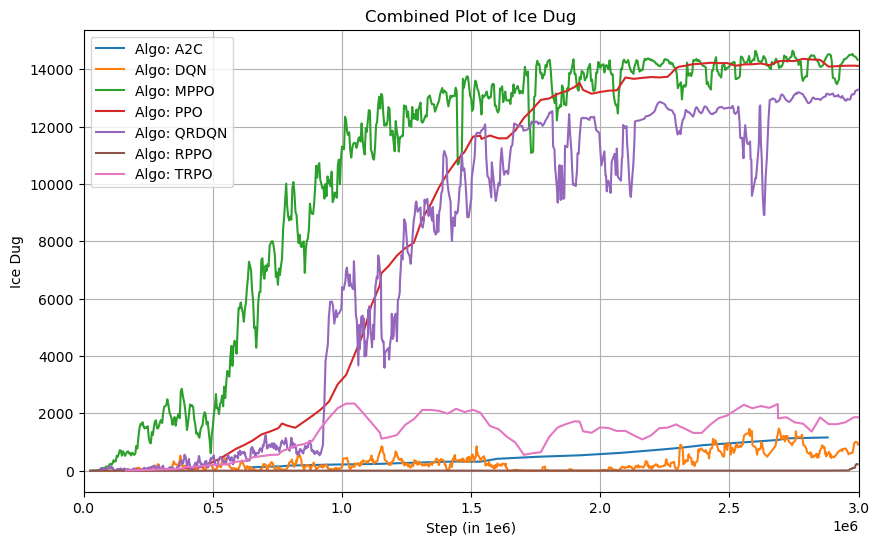
\includegraphics[width=\linewidth]{images/results_singleunit/mean_ice_total.png}
        \captionsetup{justification=justified, singlelinecheck=false, width=0.8\linewidth, labelfont=bf} 
        \caption{Average ice dug during evaluation phases throughout training.}
        \label{fig:mean-ice-total}
    \end{minipage}\hfill
    \begin{minipage}{0.5\textwidth}
        \centering
        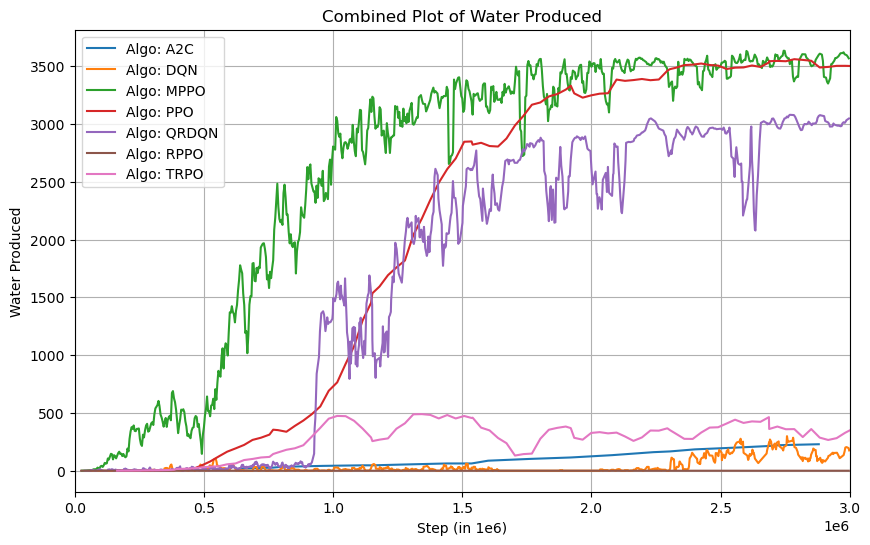
\includegraphics[width=\linewidth]{images/results_singleunit/mean_water_total.png}
        \captionsetup{justification=justified, singlelinecheck=false, width=0.9\linewidth, labelfont=bf} 
        \caption{Average water collected during evaluation phases throughout training.}
        \label{fig:mean-water-total}
    \end{minipage}
\end{figure}

\noindent \textcolor{deepblue}{\autoref{fig:mean-ice-total}} and \textcolor{deepblue}{\autoref{fig:mean-water-total}} demonstrate that PPO, M-PPO, and QR-DQN significantly outperformed all other algorithms. These plots also reveal that the performance of certain algorithms, such as A2C and DQN, has been improving, while TRPO remained stagnant in a local optimum throughout the evaluations. In stark contrast, ARS and R-PPO underperformed significantly. To further assess the models, we also considered the speed and convergence time of the algorithms to identify the most suitable one for our specific task.

\bigskip

\begin{minipage}[htbp]{0.45\textwidth}
    \centering
    \begin{tabular}{|c|c|c|}
        \hline
        \textbf{Algorithm} & \textbf{SPS} & \textbf{Convergence} \\
        \hline
        TRPO  & 1897  &  - \\
        A2C &  3032 & - \\
        \textbf{PPO}    &  \textbf{2742} & \textbf{1.6M steps} \\
        R-PPO   & 656 & - \\
        \textbf{M-PPO}  & \textbf{1258} & \textbf{1.2M steps} \\
        DQN  &  2464 & - \\
        \textbf{QR-DQN}   & \textbf{170} & \textbf{1.7M steps}\\
        ARS  & 3246 & - \\
        \hline
    \end{tabular}
    \captionsetup{justification=justified, singlelinecheck=false, width=1\linewidth, labelfont=bf} 
    \captionof{table}{Steps per second were recorded throughout training, indicating how many environmental steps in the rollout buffer could the algorithms process per second in the evaluation phases. Convergence data is missing for five of the algorithms, as they did not achieve an episode length of 1000 in any evaluation phase. In the table, we calculated steps in millions, hence the notation of \textbf{M}. \vspace{4pt}}
    \label{tab:single-agent-results-conv}
\end{minipage}%
\hfill
\begin{minipage}[htbp]{0.45\textwidth}
    \centering
    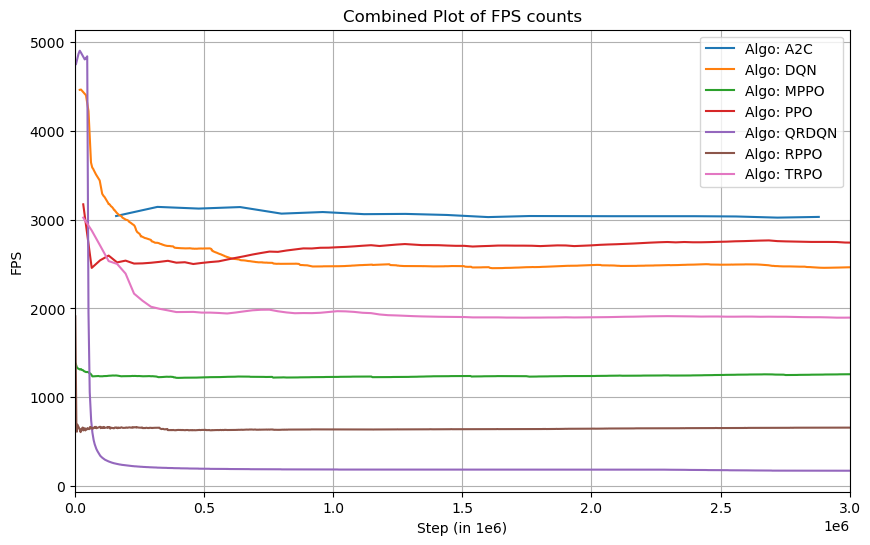
\includegraphics[width=\linewidth]{images/results_singleunit/mean_fps_total.png}
    \captionsetup{justification=justified, singlelinecheck=false, width=1\linewidth, labelfont=bf} 
    \captionof{figure}{The plot represents a running average of steps per second during evaluation phases throughout training. It is evident from the plot that the numbers eventually stabilize around a specific value, which accurately reflects the true speed of the algorithm. \vspace{26pt}}
    \label{fig:mean-sps-total}
\end{minipage}


\noindent The data in \textcolor{deepblue}{\autoref{tab:single-agent-results-conv}} validates a key assumption: masking out invalid actions in the environment, thereby limiting the exploration space, proves advantageous in early training. This approach accelerates learning by preventing illegal moves. The ongoing cost of recalculating masks in later training stages yields diminishing returns, as the model naturally learns to avoid meaningless actions over time. Nonetheless, this trade-off is highly favorable, as the early acceleration is essential to prevent the agent from getting stuck in local optima, and the minor decrease in training speed during later phases is acceptable. It's worth mentioning that QR-DQN (\autoref{sec:qrdqn}) exhibits significantly slower performance, primarily due to the utilization of 200 quantiles, which multiplies the action space by 200-fold. Consequently, the action space expands to 11 actions, resulting in an output shape for the heads of $11 \times 200 = 2200$, compared to just 11.


\section{Monolithic Approach}
\label{sec:monolithic-approach-results}

\section{Hybrid Approach}
\label{sec:hybrid-approach-results}

\noindent In this section, our primary focus will be on showcasing the effectiveness of our technique called \textbdd{trajectory separation} (\autoref{subsec:grouping}) to demonstrate its potential for improving the hybrid architecture (\autoref{sec:hybrid-approach}). In addition, we will explore potential enhancements and limitations of the method, including examining the components of trajectory separation to determine the specific factors that contribute to the improvement of performance. We will also conduct a comparative analysis between the trajectory-separated hybrid, \textbdd{pixel-to-pixel} architecture (\autoref{par:pixel-to-pixel}) and existing solutions for the Lux AI competition. At the end of the section, an ablation study will be carried out, analyzing the methods in addition to trajectory separation.

\bigskip

\noindent In the subsequent configurations, factories, and units will be organized into distinct groups, each with aggregated outputs and trajectories. Groups can exhibit various characteristics, from global groups encompassing all entities of a specific type to individual groups in which each entity functions as its own separate group. In this study, we illustrate the significance of distinct trajectories within a multi-agent setting and investigate various approaches for distributing rewards among the agents. All of the experiments shared a common training objective, which was to train the units to keep the factories alive until the end of the game, spanning 1,000 steps. In the following experiments, we will employ the metrics specified in \autoref{sec:hybrid-metrics}. These metrics include the length of an episode, the aggregate amount of ice transferred to factories within a given episode, and the count of operational factories at each environment step, normalized by the maximum episode duration.

\bigskip

\noindent The experiments consist of three separate runs, each utilizing different seeds and running for a total of 102,400 steps (25 training cycles with a 4,096-step batch size). We felt the difference between variants could be sufficiently highlighted in this step range. Contrary to the single-unit test bench (\autoref{sec:single-unit-testbench-results}) and the monolithic approach test (\autoref{sec:monolithic-approach-results}), in this scenario, both players are active and performing actions simultaneously. The same model, as detailed in \autoref{sec:hybrid-network-architecture}, was used for both players and was trained on their collective trajectories. Following each training cycle, we ran an evaluation of the model by executing 12 distinct environments until the conclusion of the matches. These environments were seeded differently for each of the three runs. The evaluation process yielded 36 data points per training cycle for environment-specific metrics, specifically the metric of \textttdb{Episode Length}. Additionally, by considering each player separately, there were 72 data points for player-specific metrics, including \textttdb{Ice Transferred} and \textttdb{Average Factory Alive}. The lines on the charts visually represent the metrics' means, while the shaded area shows the standard deviation. In addition to the charts, tables are included to make comparisons easier. The columns \textttdb{Final Ice Transferred} and \textttdb{Final Episode Length} refer to the metrics collected at the last evaluation of the model. The mean value is presented, along with the standard deviation in brackets. The \textttdb{X\% of Episodes Finished by} metrics measure how long it took for the agents to learn how to keep the factories alive until the end of the game in terms of environment steps. The percentage indicates the ratio of evaluation environments that resulted in a finished episode, which is an episode where at least one factory survived from both players until 1,000 steps.

\subsection{Trajectory separation} \label{sec:trajectory-separation}

\subsubsection{Global Trajectory vs Separated Trajectories}

\noindent An initial experiment was done to see what effect \textbdd{separated trajectories} (\autoref{subsec:grouping}) had on how fast the agents learned. As the control group, we implemented a variant that closely resembles the original pixel-to-pixel method (\cite{chen2023emergent}) by utilizing a single \textbdd{global group} (\textttdb{"single global trajectory"}), resulting in a centralized architecture. To evaluate our more decentralized approach, we experimented with various group configurations. These configurations included the formation of distinct \textbdd{global groups} for each entity type (\textttdb{"global factories, global units"}), the creation of a single global group for one entity type while maintaining individual groups for the other (\textttdb{"global factories, separate units"}, \textttdb{"separate factories, global units"}), and the establishment of \textbdd{individual groups} for each entity (\textttdb{"separate trajectories for all entities"}). As demonstrated in \autoref{fig:hybrid_results/trajectory_separation/combined} and \autoref{tab:hybrid_results/trajectory_separation/combined}, the variants with separated trajectories perform much better compared to the global trajectory variants. The most notable improvement is the rate of convergence, which resulted in learning to keep the factories alive until the end of the game by around the 50,000th step, which the fully global variant could not achieve at all. Upon arriving at this significant milestone, the agents continued to improve their strategies further, leading to an average transfer of more than 40,000 ice to factories throughout the 1,000 steps in an episode. The value is 13 times greater than the achievement of the global trajectory variant. The accomplishment was reached by acquiring the skill to transfer ice to all of the factories rather than solely to one, which would have been sufficient to reach the maximum episode length. We can see this by the \textttdb{Average Factory Alive} metric, which continues to rise even after the \textttdb{Episode Length} levels off at the maximum possible value. The new technique also reduced the frequent fluctuations of the model's performance, which hinted at unlearning the progress made by the previous steps. We suspect this was the cause of destructive behavior reinforcement, which our method avoids since agents are only rewarded for their actual work (explained in \autoref{subsec:methodcomp}). The findings of the experiment indicate that utilizing separate trajectories can offer a notable benefit to the agents' training process.

\begin{figure}[htbp]
    \centering
    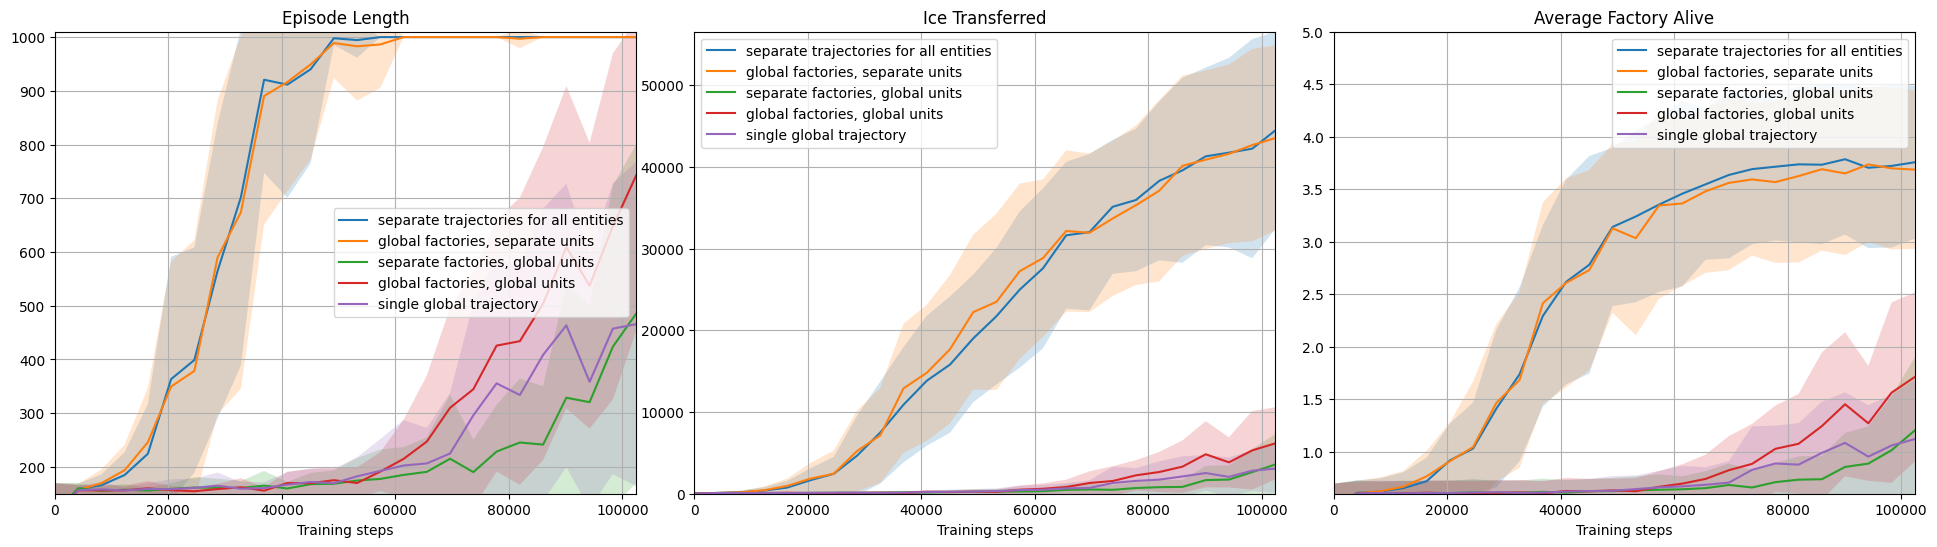
\includegraphics[width=1\linewidth]{images/results_hybrid/trajectory_separation/combined.png}
    \captionsetup{justification=justified, singlelinecheck=false, width=1\linewidth, labelfont=bf} 
    \caption[]{Plot comparing the usage of trajectory separation and global trajectories in terms of the length of the episodes, ice transferred by units, and number of active factories. The data presented in the figure indicates a clear improvement in all metrics thanks to the utilization of trajectory separation. In addition to faster convergence, the variants with separated trajectories exhibit reduced fluctuations in performance, thereby leading to more efficient training.}
    \label{fig:hybrid_results/trajectory_separation/combined}
\end{figure}

\begin{table}[htbp]
    \footnotesize
    \renewcommand{\arraystretch}{1.2}%
    \begin{tabularx}{\textwidth}{|X|C{2.3cm}|C{2.3cm}|C{2.0cm}|C{2.0cm}|}
        \hline
\multicolumn{1}{|Y|}{\textbf{Group Name}} & \textbf{Final Ice Transferred} & \textbf{Final Episode Length} & \textbf{10\% of Episodes Finished by} & \textbf{95\% of Episodes Finished by} \\
        \hline
separate trajectories for all entities & 44,472 (12,065) & 1,000 (0) & 28,672 steps & 49,152 steps \\
global factories, separate units & 43,528 (11,327) & 1,000 (0) & 28,672 steps & 49,152 steps \\
separate factories, global units & 3,573 (3,753) & 485 (315) & 98,304 steps & - \\
global factories, global units & 6,162 (4,413) & 742 (290) & 81,920 steps & - \\
single global trajectory & 3,066 (2,996) & 466 (302) & 102,400 steps & - \\
        \hline
    \end{tabularx}
    \medskip
    \captionsetup{justification=justified, singlelinecheck=false, width=1\linewidth, labelfont=bf} 
    \caption{Table comparing the usage of trajectory separation and global trajectories. The metrics featured include the amount of ice transferred by units and the length of the episodes in the evaluation phase following the last training cycle. The table also contains the observed environment steps needed until the model reaches the maximum episode length in the specified percentage of evaluation environments. The variant with completely separate trajectories was able to provide the factories with 13 times more ice after the training and has managed to reach the maximum episode length in 10\% of the evaluation environments more than 3 times faster.}
    \label{tab:hybrid_results/trajectory_separation/combined}
\end{table}

\bigskip

\subsubsection{Number of Optimal Trajectories}

\label{subsec:modulus-grouping}
\noindent In order to demonstrate the significance of separating the entity trajectories, we conducted an additional experiment in which we categorized the units into \textbdd{N} groups based on the modulus of their unique IDs. This categorization led to approximately random allocation across the groups, enabling us to examine the optimal number of trajectories to divide our training steps into. The units were the only entities involved in the grouping, as the factories remained entirely separate during this test. The results are displayed in \autoref{fig:hybrid_results/group_size/combined} and \autoref{tab:hybrid_results/group_size/combined}. It is evident that increasing the number of trajectories resulted in a faster and more efficient training process for the agents, suggesting that the optimal training method is utilizing a separate trajectory for all entities.

\begin{figure}[htbp]
    \centering
    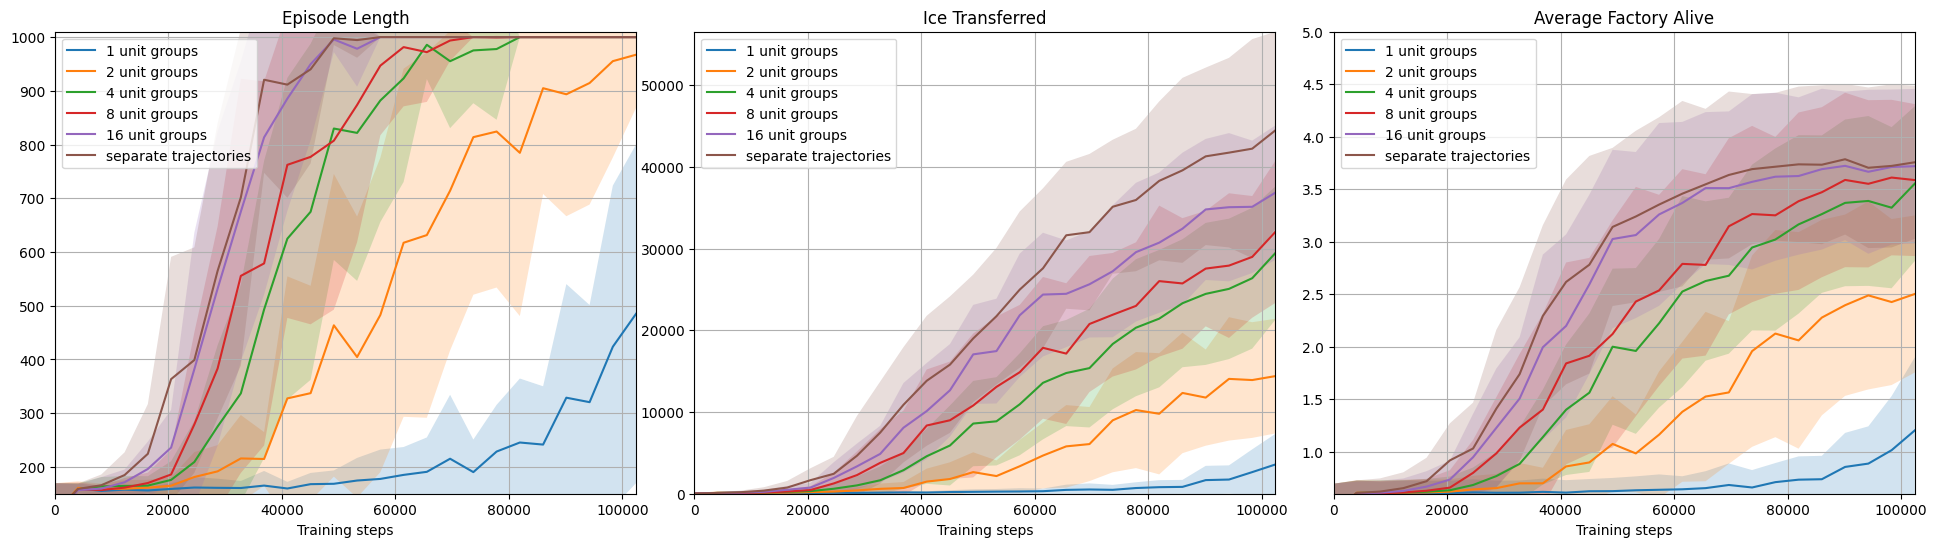
\includegraphics[width=1\linewidth]{images/results_hybrid/group_size/combined.png}
    \captionsetup{justification=justified, singlelinecheck=false, width=1\linewidth, labelfont=bf} 
    \caption[]{Plot comparing the performance of separating the global trajectory into N separate trajectories in terms of the length of the episodes, ice transferred by units, and number of active factories. In addition to the test variants, the global and completely separate trajectory variants are also present. The figure indicates a positive correlation between the number of separate trajectories and the performance achieved on all metrics.}
    \label{fig:hybrid_results/group_size/combined}
\end{figure}

\begin{table}[htbp]
    \footnotesize
    \renewcommand{\arraystretch}{1.2}%
    \begin{tabularx}{\textwidth}{|X|C{2.3cm}|C{2.3cm}|C{2.0cm}|C{2.0cm}|}
        \hline
\multicolumn{1}{|Y|}{\textbf{Group Name}} & \textbf{Final Ice Transferred} & \textbf{Final Episode Length} & \textbf{10\% of Episodes Finished by} & \textbf{95\% of Episodes Finished by} \\
        \hline
1 unit groups & 3,573 (3,753) & 485 (315) & 98,304 steps & - \\
2 unit groups & 14,388 (7,019) & 967 (99) & 57,344 steps & - \\
4 unit groups & 29,459 (8,150) & 1,000 (0) & 36,864 steps & 77,824 steps \\
8 unit groups & 32,049 (8,701) & 1,000 (0) & 32,768 steps & 61,440 steps \\
16 unit groups & 36,847 (8,224) & 1,000 (0) & 28,672 steps & 57,344 steps \\
separate trajectories & 44,472 (12,065) & 1,000 (0) & 28,672 steps & 49,152 steps \\
        \hline
    \end{tabularx}
    \medskip
    \captionsetup{justification=justified, singlelinecheck=false, width=1\linewidth, labelfont=bf} 
    \caption{Table comparing the performance of separating the global trajectory into N separate trajectories. The metrics featured include the amount of ice transferred by units and the length of the episodes in the evaluation phase following the last training cycle. The table also contains the observed environment steps needed until the model reaches the maximum episode length in the specified percentage of evaluation environments. In addition to the test variants, the global and completely separate trajectory variants are also present. The table shows a massive jump in the final average episode length even by separating the global trajectory into two random groups. While the episode length metric reaches its maximum value with 4 unit groups, an increased convergence rate can be observed by using even more separate trajectories.}
    \label{tab:hybrid_results/group_size/combined}
\end{table}


\subsection{Trajectory Number Reduction}
\label{subsec:trajec_reduc}

\noindent The technique of \textbdd{trajectory separation} (\autoref{sec:trajectory-separation}) provides an optimized approach that enables efficient training of a centralized model for a multi-agent problem. However, it should be noted that the large number of trajectories does have certain limitations. Given that the separated \textbdd{training examples} are tied to their respective environment steps, which are used to partition our \textbdd{mini-batches} during training, and considering that the number of trajectories can vary at each step, it is possible for the mini-batches to have an imbalanced number of training examples. Given that the sizes of the matrices remain constant and padding values are used for inactive groups, this does not pose any issues regarding vectorization or memory utilization. Nevertheless, this phenomenon could potentially lead to an asymmetry in the impact that each training example has on the policy loss, as the final loss is obtained by averaging all training examples. Steps with a large number of currently active groups will carry more significance, whereas the impact of a group's example within a step with a low number of active groups will be more pronounced compared to a group's example within a step with a higher population. This is because, on average, the former will be included in a mini-batch with fewer examples. Even if the mini-batch sizes were balanced, it would remain uncertain whether the increased number of trajectories is advantageous for the training process. The generation of a large number of training instances from the available environment steps introduces a regularization effect to the model's training process, thereby reducing the influence of each individual instance. If the primary challenge associated with a single global trajectory is the complex action space and the incomprehensible singular reward value, it is possible that by eliminating these factors, a reduced quantity of training examples may be sufficient to obtain convergence. Reducing the size of the batches while maintaining the same performance would further optimize our technique. In order to assess the impact of the aforementioned issues, we will employ two methodologies: agent grouping, wherein we will evaluate the performance attainable through various grouping criteria, and trajectory sample reduction, wherein we will selectively utilize data from the top or bottom N groups based on a specified metric for each step in the environment.

\subsubsection{Grouping}

\noindent The results of the modulus test in \autoref{subsec:modulus-grouping} show a strong link between performance and the number of allowed separate trajectories. The variant that was unconstrained by any kind of grouping outperformed all the other variants. However, it raises the question of whether comparable performance can be attained with a bounded variant by implementing a grouping rule that is beneficial for the training process. As shown in \autoref{fig:hybrid_results/group_rule/combined} and \autoref{tab:hybrid_results/group_rule/combined}, our experiment involved evaluating the effectiveness of three different grouping strategies: grouping by map segments, grouping by closest factories, and grouping by closest heavy units. All of these groupings led to a bounded number of trajectories, as the size of the map remains constant, and the number of factories can only vary between three and five. At first glance, the number of heavy units may appear to be limitless; however, the resources available to a factory only permit the production of a single heavy unit per factory. None of the groups that were tested were able to achieve performance comparable to that of the completely separated variant. Additionally, the number of groups remained a significant indicator of performance. We used the variants from \autoref{fig:hybrid_results/group_size/combined} to see if non-random grouping rules can do better than a random group assignment with the same number of separated groups. Unfortunately, all of the variants that were subjected to testing demonstrated lower performance or demonstrated comparable results to those assigned randomly. The sole exception was the \textttdb{"closest heavy"}; however, it still failed to outperform random assignment in terms of converging to the maximum episode length. The findings indicate that the approach of grouping the trajectories of entities together in order to reduce the number of training examples yields poor performance.

\begin{figure}[htbp]
    \centering
    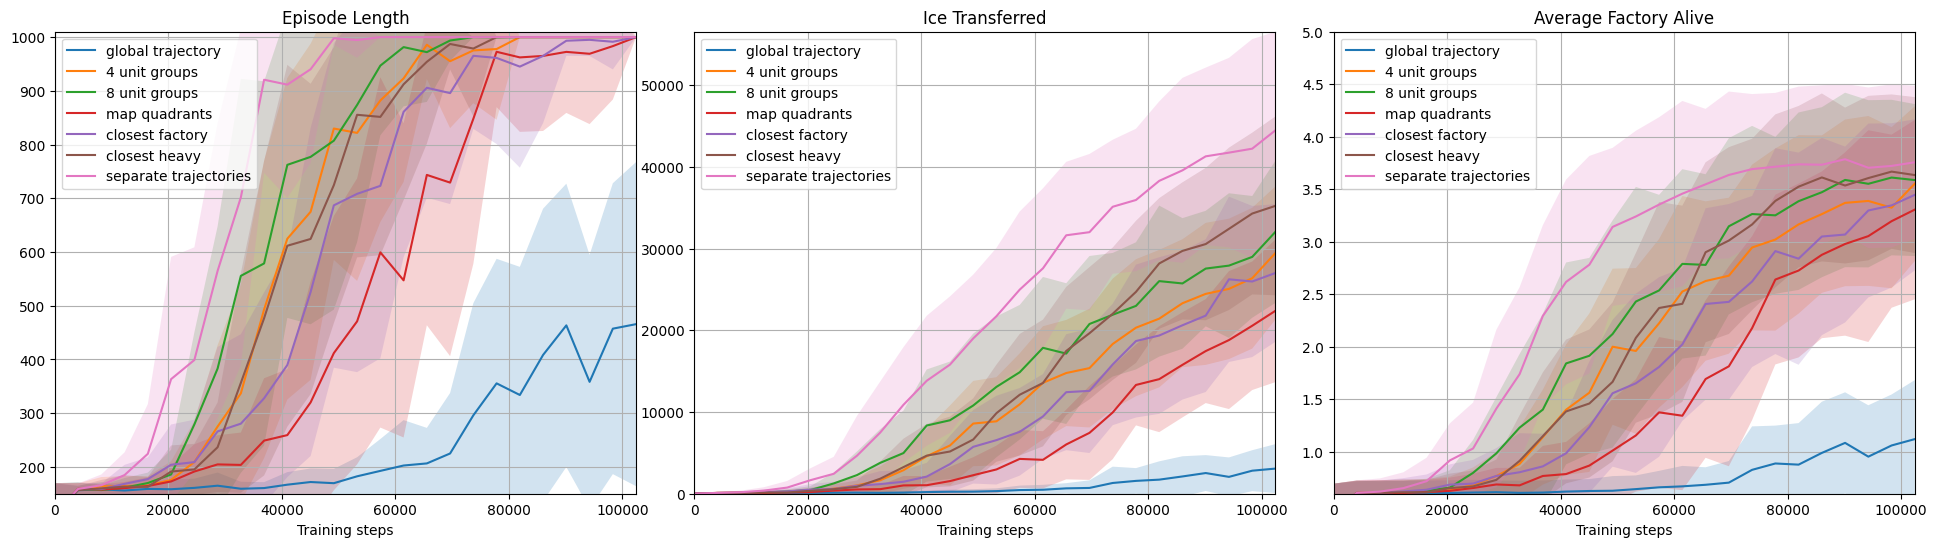
\includegraphics[width=1\linewidth]{images/results_hybrid/group_rule/combined.png}
    \captionsetup{justification=justified, singlelinecheck=false, width=1\linewidth, labelfont=bf} 
    \caption[]{Plot comparing the usage of different grouping rules in terms of the length of the episodes, ice transferred by units, and number of active factories. In addition to the test variants, the global and completely separate trajectory variants are also present. None of the tried variants managed to beat the separate trajectory variant in performance.}
    \label{fig:hybrid_results/group_rule/combined}
\end{figure}

\begin{table}[htbp]
    \footnotesize
    \renewcommand{\arraystretch}{1.2}%
    \begin{tabularx}{\textwidth}{|X|C{2.3cm}|C{2.3cm}|C{2.0cm}|C{2.0cm}|}
        \hline
\multicolumn{1}{|Y|}{\textbf{Group Name}} & \textbf{Final Ice Transferred} & \textbf{Final Episode Length} & \textbf{10\% of Episodes Finished by} & \textbf{95\% of Episodes Finished by} \\
        \hline
global trajectory & 3,066 (2,996) & 466 (302) & 102,400 steps & - \\
4 unit groups & 29,459 (8,150) & 1,000 (0) & 36,864 steps & 77,824 steps \\
8 unit groups & 32,049 (8,701) & 1,000 (0) & 32,768 steps & 61,440 steps \\
map quadrants & 22,385 (8,733) & 1,000 (0) & 53,248 steps & 98,304 steps \\
closest factory & 27,009 (8,420) & 1,000 (0) & 45,056 steps & 94,208 steps \\
closest heavy & 35,224 (10,946) & 1,000 (0) & 36,864 steps & 73,728 steps \\
separate trajectories & 44,472 (12,065) & 1,000 (0) & 28,672 steps & 49,152 steps \\
        \hline
    \end{tabularx}
    \medskip
    \captionsetup{justification=justified, singlelinecheck=false, width=1\linewidth, labelfont=bf} 
    \caption{Table comparing the usage of different grouping rules. The metrics featured include the amount of ice transferred by units and the length of the episodes in the evaluation phase following the last training cycle. The table also contains the observed environment steps needed until the model reaches the maximum episode length in the specified percentage of evaluation environments. In addition to the test variants, the global and completely separate trajectory variants are also present. While each grouping configuration performed better than the global trajectory variant, none could compete with the convergence rate of the completely separate trajectory variant. Grouping units by specific rules did not perform better than random grouping.}
    \label{tab:hybrid_results/group_rule/combined}
\end{table}

\subsubsection{Train Sample Reduction}
\label{subsec:tsr}

\noindent Given that all grouping methods performed less effectively than completely separate trajectories for all entities, we attempted an alternative approach to ensure a more consistent number of training examples at each step. Our technique, referred to as \textbdd{train sample reduction}, involves selecting the top N examples from each step and training the model exclusively on those chosen examples. This action accomplishes two objectives. Firstly, it establishes an \textbdd{upper limit for the train examples}, thereby ensuring that the influence of each group's action remains relatively consistent, regardless of the number of other active groups. Secondly, in theory, by selecting only the most relevant examples at each step, we should be capable of \textbdd{accelerating the training process} of the model in terms of the number of environment steps and the amount of time required. In the following experiments, we utilize completely separated trajectories for all variants and perform the sample reduction solely on the train examples of units.

\bigskip

\noindent In order to first determine the optimal metric for selecting the desired subset of examples by, we conducted an experiment. We tried selecting the top N=1 samples by using various sampling techniques, including \textbdd{random sampling}, \textbdd{top advantage value}, \textbdd{top absolute advantage value} and \textbdd{top return value}. Among all of these variations, the subset that includes the examples with the greatest advantage value achieved the highest performance, as evidenced by the results presented in \autoref{fig:hybrid_results/trajectory_sample_reduction/combined} and \autoref{tab:hybrid_results/trajectory_sample_reduction/combined}. Interestingly, utilizing solely the example with the \textbdd{most prominent advantage value} exhibited \textbdd{almost the same performance} as employing all of the train examples. Consequently, we decided to investigate sampling by this metric further, with different N values.

\begin{figure}[htbp]
    \centering
    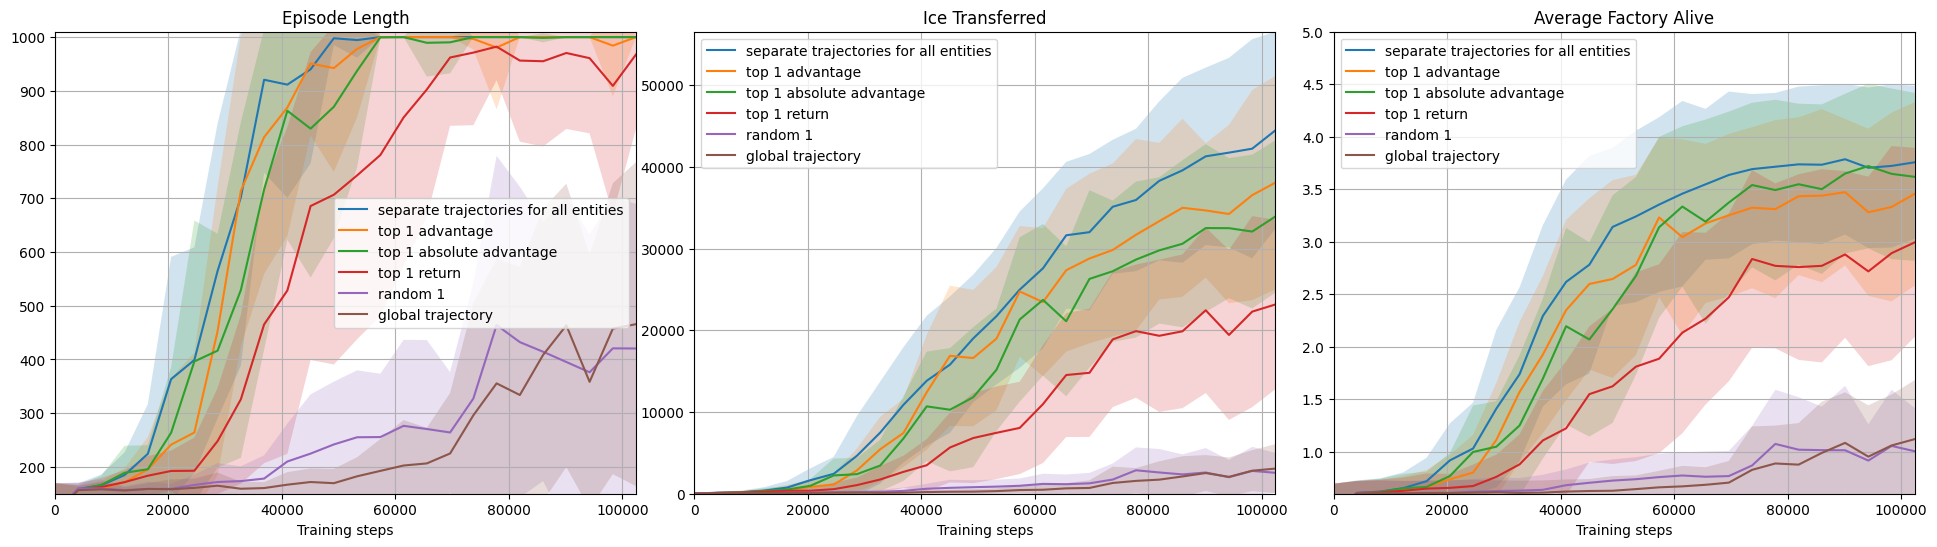
\includegraphics[width=1\linewidth]{images/results_hybrid/trajectory_sample_reduction/combined.png}
    \captionsetup{justification=justified, singlelinecheck=false, width=1\linewidth, labelfont=bf} 
    \caption[]{Plot comparing the different methods of trajectory sample reduction in terms of the length of the episodes, ice transferred by units, and number of active factories. In addition to the test variants, the global and completely separate trajectory variants are also present. Randomly selecting a single example at each step has the same effect as using a global trajectory. Out of all the sampling methods tried, selecting by advantage is the most prominent, leading to almost the same performance as using all data.}
    \label{fig:hybrid_results/trajectory_sample_reduction/combined}
\end{figure}

\begin{table}[htbp]
    \footnotesize
    \renewcommand{\arraystretch}{1.2}%
    \begin{tabularx}{\textwidth}{|X|C{2.3cm}|C{2.3cm}|C{2.0cm}|C{2.0cm}|}
        \hline
\multicolumn{1}{|Y|}{\textbf{Group Name}} & \textbf{Final Ice Transferred} & \textbf{Final Episode Length} & \textbf{10\% of Episodes Finished by} & \textbf{95\% of Episodes Finished by} \\
        \hline
separate trajectories for all entities & 44,472 (12,065) & 1,000 (0) & 28,672 steps & 49,152 steps \\
top 1 advantage & 38,072 (13,071) & 1,000 (0) & 32,768 steps & 57,344 steps \\
top 1 absolute advantage & 33,926 (9,324) & 1,000 (0) & 32,768 steps & 57,344 steps \\
top 1 return & 23,156 (10,369) & 968 (138) & 40,960 steps & - \\
random 1 & 2,550 (2,434) & 420 (269) & 77,824 steps & - \\
global trajectory & 3,066 (2,996) & 466 (302) & 102,400 steps & - \\
        \hline
    \end{tabularx}
    \medskip
    \captionsetup{justification=justified, singlelinecheck=false, width=1\linewidth, labelfont=bf} 
    \caption{Table comparing the different methods of trajectory sample reduction. The metrics featured include the amount of ice transferred by units and the length of the episodes in the evaluation phase following the last training cycle. The table also contains the observed environment steps needed until the model reaches the maximum episode length in the specified percentage of evaluation environments. In addition to the test variants, the global and completely separate trajectory variants are also present. The table shows how selecting a single train example from each step by the right metric could approximate the training performance on all data. The advantage value proved to be the best metric for sampling.}
    \label{tab:hybrid_results/trajectory_sample_reduction/combined}
\end{table}

\bigskip

\noindent We tested the impact of selecting different numbers of examples with the highest advantage values from each environment step. Specifically, we tested the effects of taking 1, 2, 4, 8, and 16 such examples. The results are presented in \autoref{fig:hybrid_results/trajectory_sample_reduction_advantage/combined} and \autoref{tab:hybrid_results/trajectory_sample_reduction_advantage/combined}. Curiously, the inclusion of additional examples does not appear to significantly enhance performance. In fact, the performance is slightly hindered when the sample size is increased to 16. This implies that the significance of an entity's action may be diminished by the multitude of other actions currently occurring in the surrounding environment, making the action less dominant in the loss calculation. By reducing the number of separate training examples and subsequently removing unnecessary data beforehand, we can help the convergence of the model. The slight edge exhibited by the sampled variants could also potentially be attributed to avoiding the problem of changing batch sizes, although a definitive conclusion cannot be drawn.

\begin{figure}[htbp]
    \centering
    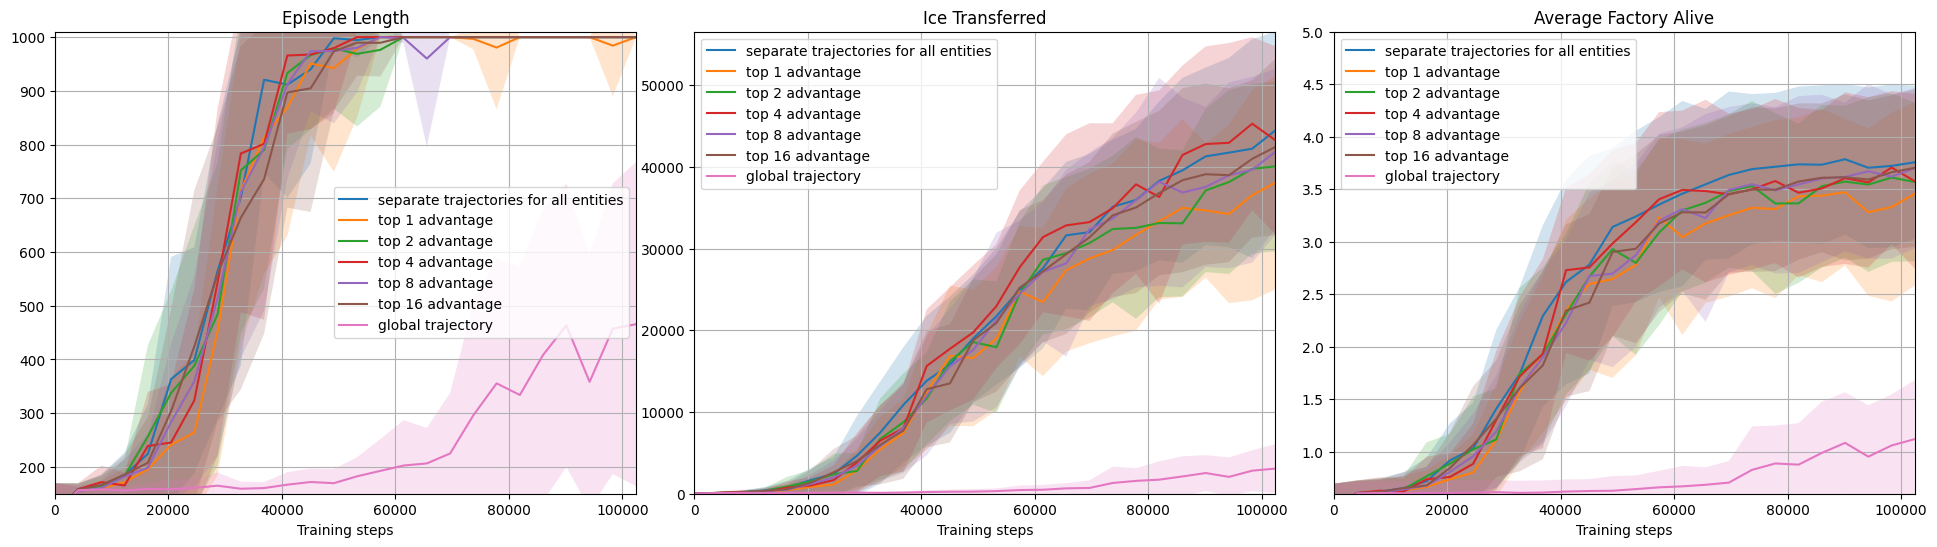
\includegraphics[width=1\linewidth]{images/results_hybrid/trajectory_sample_reduction_advantage/combined.png}
    \captionsetup{justification=justified, singlelinecheck=false, width=1\linewidth, labelfont=bf} 
    \caption[]{Plot comparing the performance of sampling train examples based on the advantage values in terms of the length of the episodes, ice transferred by units, and number of active factories. In addition to the test variants, the global and completely separate trajectory variants are also present. Increasing the number of sampled values appears to have minimal effect on performance, leading us to believe that the main benefit of utilizing a larger training set is to find outstandingly beneficial examples.}
    \label{fig:hybrid_results/trajectory_sample_reduction_advantage/combined}
\end{figure}

\begin{table}[htbp]
    \footnotesize
    \renewcommand{\arraystretch}{1.2}%
    \begin{tabularx}{\textwidth}{|X|C{2.3cm}|C{2.3cm}|C{2.0cm}|C{2.0cm}|}
        \hline
\multicolumn{1}{|Y|}{\textbf{Group Name}} & \textbf{Final Ice Transferred} & \textbf{Final Episode Length} & \textbf{10\% of Episodes Finished by} & \textbf{95\% of Episodes Finished by} \\
        \hline
separate trajectories for all entities & 44,472 (12,065) & 1,000 (0) & 28,672 steps & 49,152 steps \\
top 1 advantage & 38,072 (13,071) & 1,000 (0) & 32,768 steps & 57,344 steps \\
top 2 advantage & 40,053 (10,402) & 1,000 (0) & 24,576 steps & 61,440 steps \\
top 4 advantage & 43,246 (11,518) & 1,000 (0) & 28,672 steps & 49,152 steps \\
top 8 advantage & 41,855 (10,159) & 1,000 (0) & 28,672 steps & 57,344 steps \\
top 16 advantage & 42,433 (10,792) & 1,000 (0) & 24,576 steps & 53,248 steps \\
global trajectory & 3,066 (2,996) & 466 (302) & 102,400 steps & - \\
        \hline
    \end{tabularx}
    \medskip
    \captionsetup{justification=justified, singlelinecheck=false, width=1\linewidth, labelfont=bf} 
    \caption{Table comparing the performance of sampling train examples based on the advantage values. The metrics featured include the amount of ice transferred by units and the length of the episodes in the evaluation phase following the last training cycle. The table also contains the observed environment steps needed until the model reaches the maximum episode length in the specified percentage of evaluation environments. In addition to the test variants, the global and completely separate trajectory variants are also present. Increasing the number of advantage-sampled values did not appear to have a significant effect on performance.}
    \label{tab:hybrid_results/trajectory_sample_reduction_advantage/combined}
\end{table}

\bigskip

\noindent We were also interested in investigating the performance that can be achieved through random sampling. We conducted an experiment examining the performance of different numbers of random samples, specifically 1, 2, 4, 8, and 16. The aforementioned variants were subsequently compared to the established, completely separate, and global variants. The results are available in \autoref{fig:hybrid_results/trajectory_sample_reduction_random/combined} and \autoref{tab:hybrid_results/trajectory_sample_reduction_random/combined}. Using a random sampling approach cannot provide comparable performance to utilizing the entire dataset. As expected, the performance improved as we increased the number of sampled examples, consistent with the random grouping observed in the trajectory separation experiment (\autoref{subsec:modulus-grouping}).

\begin{figure}[htbp]
    \centering
    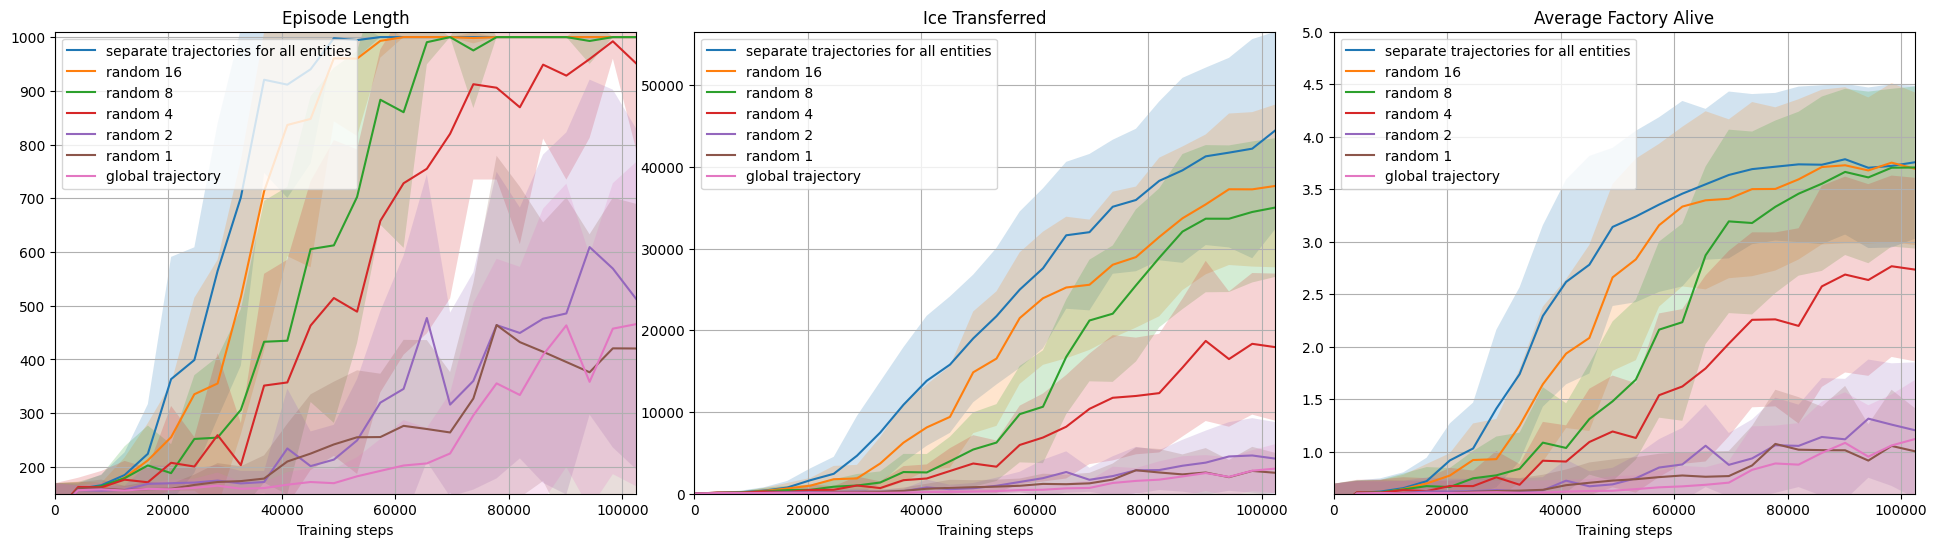
\includegraphics[width=1\linewidth]{images/results_hybrid/trajectory_sample_reduction_random/combined.png}
    \captionsetup{justification=justified, singlelinecheck=false, width=1\linewidth, labelfont=bf} 
    \caption[]{Plot showcasing the performance of random train example sampling in terms of the length of the episodes, ice transferred by units, and number of active factories. In addition to the test variants, the global and completely separate trajectory variants are also present. As expected, more randomly sampled trajectories caused better performance.}
    \label{fig:hybrid_results/trajectory_sample_reduction_random/combined}
\end{figure}

\begin{table}[htbp]
    \footnotesize
    \renewcommand{\arraystretch}{1.2}%
    \begin{tabularx}{\textwidth}{|X|C{2.3cm}|C{2.3cm}|C{2.0cm}|C{2.0cm}|}
        \hline
\multicolumn{1}{|Y|}{\textbf{Group Name}} & \textbf{Final Ice Transferred} & \textbf{Final Episode Length} & \textbf{10\% of Episodes Finished by} & \textbf{95\% of Episodes Finished by} \\
        \hline
separate trajectories for all entities & 44,472 (12,065) & 1,000 (0) & 28,672 steps & 49,152 steps \\
random 16 & 37,665 (9,965) & 1,000 (0) & 32,768 steps & 61,440 steps \\
random 8 & 35,022 (8,492) & 1,000 (0) & 45,056 steps & 69,632 steps \\
random 4 & 17,927 (9,007) & 951 (160) & 45,056 steps & - \\
random 2 & 4,284 (4,475) & 513 (317) & 77,824 steps & - \\
random 1 & 2,550 (2,434) & 420 (269) & 77,824 steps & - \\
global trajectory & 3,066 (2,996) & 466 (302) & 102,400 steps & - \\
        \hline
    \end{tabularx}
    \medskip
    \captionsetup{justification=justified, singlelinecheck=false, width=1\linewidth, labelfont=bf} 
    \caption{Table showcasing the performance of random train example sampling. The metrics featured include the amount of ice transferred by units and the length of the episodes in the evaluation phase following the last training cycle. The table also contains the observed environment steps needed until the model reaches the maximum episode length in the specified percentage of evaluation environments. In addition to the test variants, the global and completely separate trajectory variants are also present. As expected, more sampled trajectories resulted in better performance.}
    \label{tab:hybrid_results/trajectory_sample_reduction_random/combined}
\end{table}

\subsubsection{Emphasizing Data Quality over Quantity}
\noindent In \autoref{subsec:tsr}, we observed that the act of sampling a single training example from an environment step with separate trajectories yields the same suboptimal outcome as utilizing a global trajectory. Moreover, employing a sample selection method based on a reward-like metric can yield comparable performance to training on the entire dataset. From our perspective, this suggests the significance of data quality over data quantity. In order to further examine this concept, we conducted a comparison between \textbdd{train sample reduction} and \textbdd{random grouping} (\autoref{subsec:modulus-grouping}). The results are presented in \autoref{fig:hybrid_results/grouping_vs_tsr/combined} and \autoref{tab:hybrid_results/grouping_vs_tsr/combined}. In this study, the two observed methods of training sample reduction were random sampling, since it is the most easily comparable to random grouping, and advantage-based selection, which achieved the best performance in the trajectory separation test (\autoref{subsec:tsr}). We can derive from these charts that increasing the number of training examples does not necessarily lead to improved performance, as advantage-based selection managed to beat random sampling even with a smaller sample size. This shows that the primary purpose of using a large amount of data in reinforcement learning is to identify actions that are clearly more favorable. In the experiment, both grouping and trajectory separation resulted in a maximum of 4 training examples per environment step. However, it is important to note that grouping incorporates data from all entities, although it poses challenges in terms of learnability, as discussed in \autoref{subsec:methodcomp}. This increased complexity of the training data leads to a significant decrease in performance, to the extent that even random sampling, which only includes a small subset of all entity data, can achieve similar performance. Furthermore, when we switch to advantage-based sampling, which learns only from the pre-selected most relevant examples, its training massively outperforms the grouped variant's. This further confirms the significance of data quality.

\begin{figure}[htbp]
    \centering
    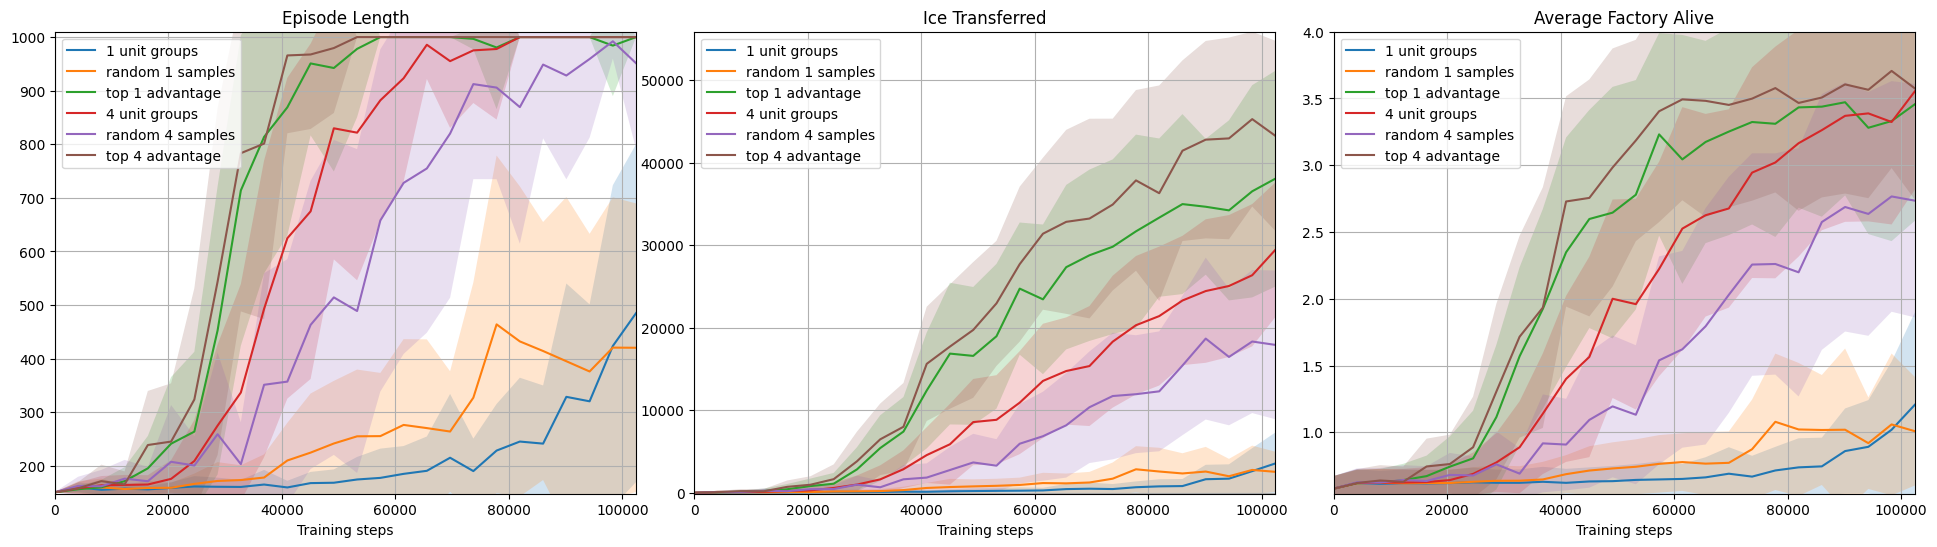
\includegraphics[width=1\linewidth]{images/results_hybrid/grouping_vs_tsr/combined.png}
    \captionsetup{justification=justified, singlelinecheck=false, width=1\linewidth, labelfont=bf} 
    \caption[]{Plot comparing random grouping, random sampling, and advantage-based sampling in terms of the length of the episodes, ice transferred by units, and number of active factories. Sampling by advantage outperforms both random grouping and random sampling, even if the advantage-based sampling contains fewer trajectories, suggesting greater importance of data quality than quantity.}
    \label{fig:hybrid_results/grouping_vs_tsr/combined}
\end{figure}

\begin{table}[htbp]
    \footnotesize
    \renewcommand{\arraystretch}{1.2}%
    \begin{tabularx}{\textwidth}{|X|C{2.3cm}|C{2.3cm}|C{2.0cm}|C{2.0cm}|}
        \hline
\multicolumn{1}{|Y|}{\textbf{Group Name}} & \textbf{Final Ice Transferred} & \textbf{Final Episode Length} & \textbf{10\% of Episodes Finished by} & \textbf{95\% of Episodes Finished by} \\
        \hline
1 unit groups & 3,573 (3,753) & 485 (315) & 98,304 steps & - \\
random 1 samples & 2,550 (2,434) & 420 (269) & 77,824 steps & - \\
top 1 advantage & 38,072 (13,071) & 1,000 (0) & 32,768 steps & 57,344 steps \\
4 unit groups & 29,459 (8,150) & 1,000 (0) & 36,864 steps & 77,824 steps \\
random 4 samples & 17,927 (9,007) & 951 (160) & 45,056 steps & - \\
top 4 advantage & 43,246 (11,518) & 1,000 (0) & 28,672 steps & 49,152 steps \\
        \hline
    \end{tabularx}
    \medskip
    \captionsetup{justification=justified, singlelinecheck=false, width=1\linewidth, labelfont=bf} 
    \caption{Table comparing random grouping, random sampling, and advantage-based sampling. The metrics featured include the amount of ice transferred by units and the length of the episodes in the evaluation phase following the last training cycle. The table also contains the observed environment steps needed until the model reaches the maximum episode length in the specified percentage of evaluation environments. The advantage-based sampling managed to outperform the other variants in all metrics, even with fewer training examples, while the random sampling underperformed random grouping.}
    \label{tab:hybrid_results/grouping_vs_tsr/combined}
\end{table}


\subsection{Method Components}
\label{subsec:methodcomp}

\noindent Although the results obtained in \autoref{sec:trajectory-separation} seem impressive, it is challenging to identify the specific factor that has led to such a substantial improvement in performance. Based on our current understanding, the act of separating the trajectories leads to four notable enhancements in the training process. The process generates additional \textbdd{training examples} from the same environmental steps, thereby enhancing the model's ability to acquire broader policies at an accelerated rate through increased exploration. Another, perhaps the most noteworthy advantage, is the eradication of the \textbdd{reinforcement of undesirable behavior}. Such reinforcement could arise if one entity performs an action that results in a high advantage value while another entity behaves in a manner that is suboptimal for the team's success but doesn't get punished by enough negative advantage. In this case, the incorrect action would be reinforced alongside the positive action. By employing separate trajectories with \textbdd{localized rewards}, the occurrence of such events can be prevented. Our method also avoids calculating advantage from steps where the original performing entity is no longer active. If only a single trajectory were utilized, there would be no way to keep track of the status and reward of individual entities. Within highly dynamic environments, such as Lux, this phenomenon leads to a somewhat misleading calculation due to the significant probability that the units and factories currently in existence will not persist until the conclusion of the episode. Consequently, it is impossible to determine whether their actions in the present have truly contributed to any real advantage. By keeping the rewards separate, we ensure that the entity receives credit for its immediate and observable efforts, both in the present and future. Lastly, separate trajectories result in separate \textbdd{advantage} calculations and separate \textbdd{critic value} outputs for all groups. Estimating the entire game state in order to provide a final global value is a significantly more complex task for the model compared to predicting multiple values based on local observations. Within this subsection, we examine the different components of trajectory separation to determine which part has the greatest impact on enhancing performance.

\subsubsection{Inividual Components}
\label{subsec:individual-components}

\noindent We initiated the study by performing a limited ablation analysis on the trajectory separation technique. Our initial hypothesis was that the most crucial components that needed to be separated were the \textbdd{reward}, \textbdd{terminal state} indication, \textbdd{critic value}, \textbdd{log probabilities}, and \textbdd{entropy} values. Therefore, we conducted a series of experiments where we systematically removed the separation of these components one by one. The purpose of these experiments was to observe the impact of each component's loss on the model's overall performance.

\bigskip

\noindent Both the \textbdd{reward} and \textbdd{critic} values are essential for the computation of the \textbdd{advantage}, an integral component of the Proximal Policy Optimization (\autoref{sec:ppo}) algorithm. Therefore, we decided to start with removing separation between these values. The results can be seen in \autoref{fig:hybrid_results/components/combined_rew} and \autoref{tab:hybrid_results/components/combined_rew}. The metrics for the \textttdb{"separate trajectories, global reward"} variant indicate that the utilization of separate trajectories with global rewards leads to a notable decrease in convergence speed, in comparison to separate trajectories with \textbdd{localized rewards}. This negative effect was expected since the absence of separated rewards hinders the model's ability to identify the specific actions undertaken by the units and factories that led to the rewards received. Consequently, this issue aligns with the problem outlined in \autoref{par:global-rew}. In order to achieve efficient global advantage calculation, the critic head of the model must learn how to predict the performance of the entire team rather than solely relying on predictions based on the local observations of individual entities. The decline in performance due to losing the ability to calculate \textbdd{critic value} predictions based on local information is further indicated by the \textttdb{"separate trajectories, global critic"} variant. The agents were able to sustain the operation of the factories for up to 1,000 steps in most environments, albeit at a slower pace, demonstrating how harder it is for the model to work solely from global information. Only when we remove both the \textbdd{critic values} and \textbdd{rewards} in test \textttdb{"separate trajectories, global advantage"} do we observe a reduction in performance to the level of a single global trajectory. A fully global \textbdd{advantage} calculation results in the same advantage value output for all entities, meaning there is no way to differentiate between positive and negative actions under the same step, massively slowing down the training. Following this modification, the only difference in the policy loss between the entities is the \textbdd{probability ratios}, which fail to provide us any information about the desired direction and magnitude of policy updates. Due to the abovementioned factors, we believe that separate rewards hold significant importance. The impact of their effect is further examined in \autoref{subsubsec:rewardass}.

\bigskip

\noindent The outcomes following the elimination of the remaining separation components, namely the termination flags and the action probabilities, are observable in \autoref{fig:hybrid_results/components/combined_misc} and \autoref{tab:hybrid_results/components/combined_misc}. The fact that the performance remained consistent even after the removal of the separated \textttdb{terminal state flags} was unexpected and surprising to us. This group can be seen under the name \textttdb{"separate trajectories, global dones"}. Given that the trajectories are separated, and only currently active entities receive rewards, indicating episode terminations prematurely at the destruction of an entity is somewhat redundant since there will be no future rewards assigned to them that could skew the return calculation anyway. The act of indicating the inactivity of a group of agents is more logical in situations where the group has the potential to become active once again, particularly in cases where multiple entities are present within the same group. If all entities within the group are destroyed, but subsequently, a new entity is assigned, it is possible for the group to regain its activity. Whether stopping the future reward calculation between these two group states is beneficial is yet to be explored. The separation of distribution entropy values does not appear to have any significance, as these values are ultimately combined into a single value to calculate the entropy loss regularization term. What massively degraded performance, however, was the removal of the separated log probabilities. Through the aggregation of log probabilities, the gradients can propagate across the action calculations of all entities. Similarly to the combined advantage value, this global gradient propagation causes weight adjustments based on the whole team's performance, making it impossible to separate individual contributions. This observation shows the necessity of utilizing separate action probabilities in order to achieve optimal training.

\begin{figure}[htbp]
    \centering
    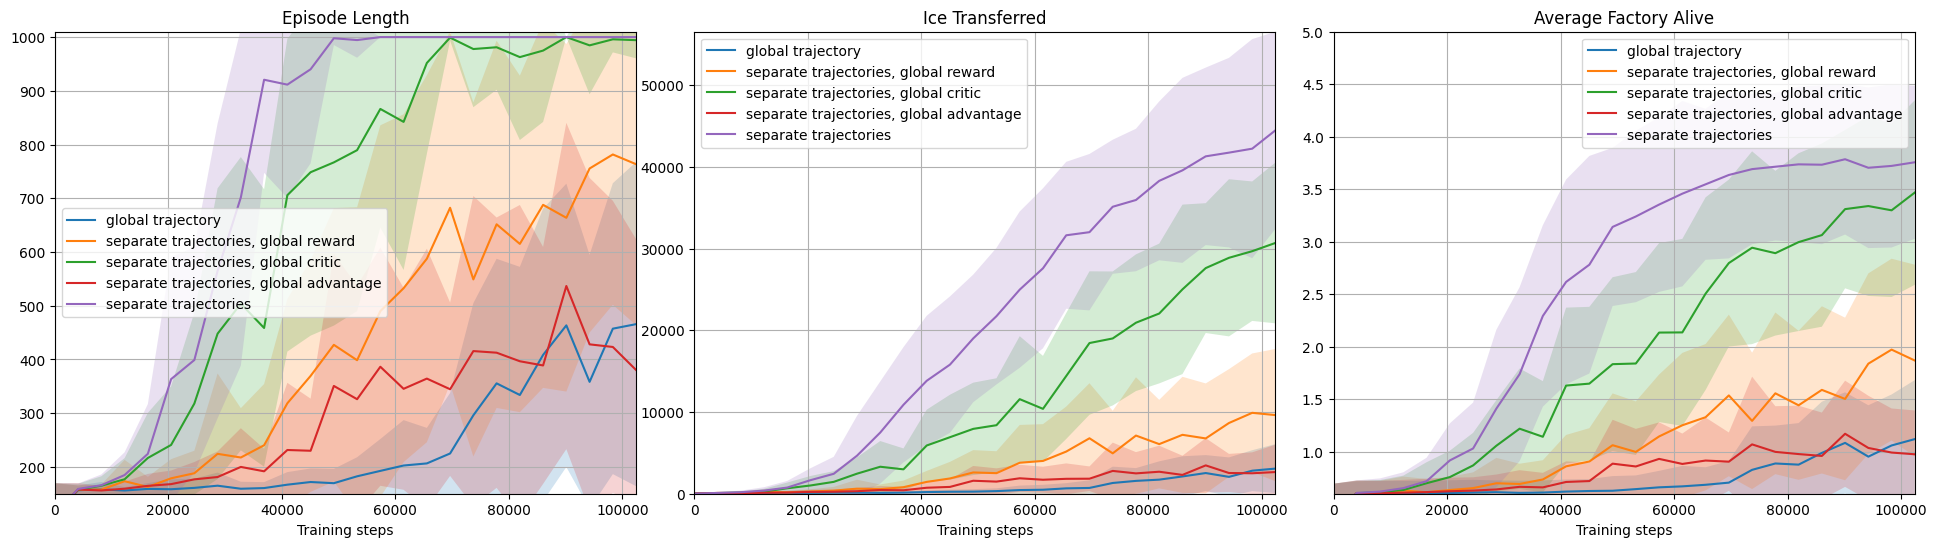
\includegraphics[width=1\linewidth]{images/results_hybrid/components/combined_rew.png}
    \captionsetup{justification=justified, singlelinecheck=false, width=1\linewidth, labelfont=bf} 
    \caption[]{Plot comparing the removal of separated components relevant to the advantage calculation in terms of the length of the episodes, ice transferred by units, and number of active factories. In addition to the test variants, the global and completely separate trajectory variants are also present. The separated reward plays a significant role but doesn't account for the whole performance boost. Removing separated critic value predictions and separated rewards together results in a similar performance to a single global trajectory.}
    \label{fig:hybrid_results/components/combined_rew}
\end{figure}

\begin{table}[htbp]
    \footnotesize
    \renewcommand{\arraystretch}{1.2}%
    \begin{tabularx}{\textwidth}{|X|C{2.3cm}|C{2.3cm}|C{2.0cm}|C{2.0cm}|}
        \hline
\multicolumn{1}{|Y|}{\textbf{Group Name}} & \textbf{Final Ice Transferred} & \textbf{Final Episode Length} & \textbf{10\% of Episodes Finished by} & \textbf{95\% of Episodes Finished by} \\
        \hline
global trajectory & 3,066 (2,996) & 466 (302) & 102,400 steps & - \\
separate trajectories, global reward & 9,614 (8,094) & 763 (300) & 53,248 steps & - \\
separate trajectories, global critic & 30,687 (9,844) & 994 (34) & 40,960 steps & 69,632 steps \\
separate trajectories, global advantage & 2,643 (3,353) & 380 (244) & 73,728 steps & - \\
separate trajectories & 44,472 (12,065) & 1,000 (0) & 28,672 steps & 49,152 steps \\
        \hline
    \end{tabularx}
    \medskip
    \captionsetup{justification=justified, singlelinecheck=false, width=1\linewidth, labelfont=bf} 
    \caption{Table comparing the removal of separated components relevant to the advantage calculation. The metrics featured include the amount of ice transferred by units and the length of the episodes in the evaluation phase following the last training cycle. The table also contains the observed environment steps needed until the model reaches the maximum episode length in the specified percentage of evaluation environments. In addition to the test variants, the global and completely separate trajectory variants are also present. Removing the separation of rewards and critic values caused a significant performance decrease. Reward appears to be the most important component.}
    \label{tab:hybrid_results/components/combined_rew}
\end{table}

\begin{figure}[htbp]
    \centering
    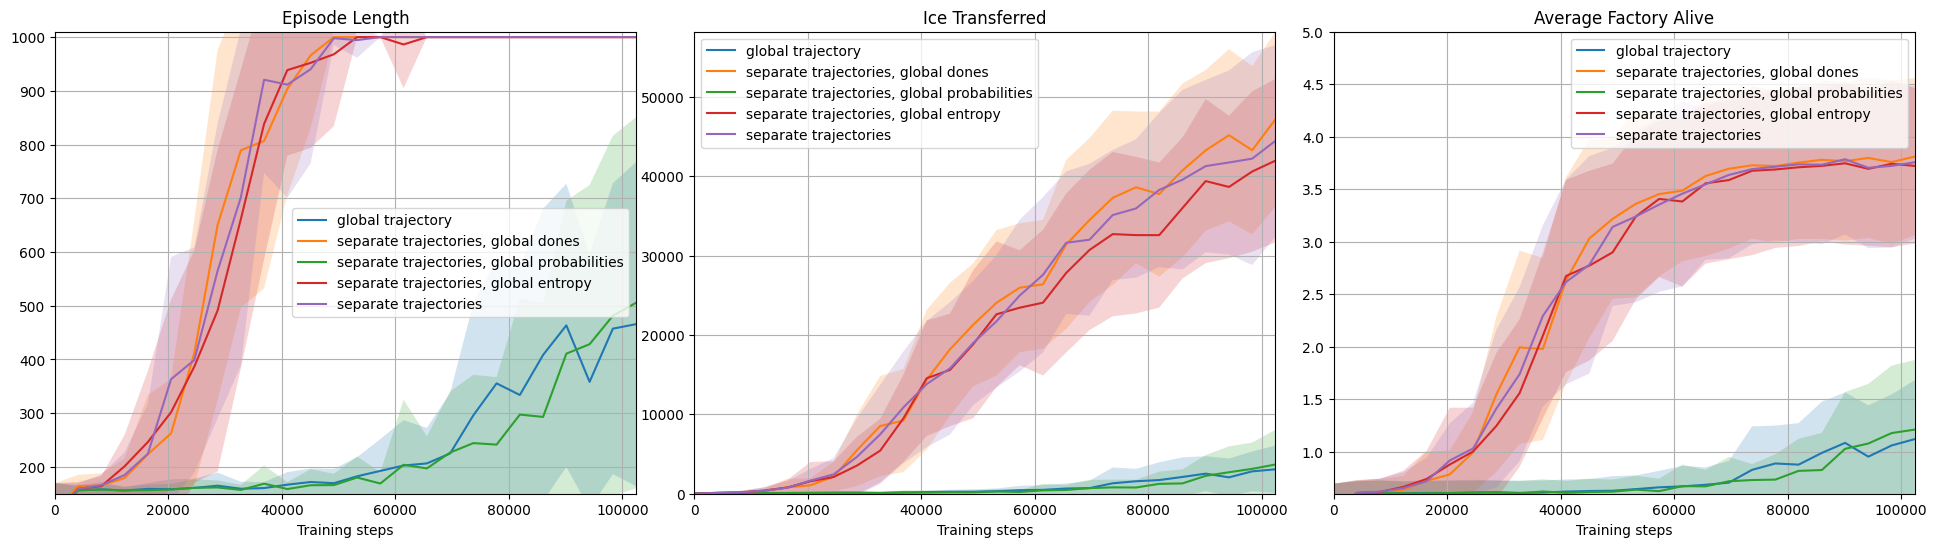
\includegraphics[width=1\linewidth]{images/results_hybrid/components/combined_misc.png}
    \captionsetup{justification=justified, singlelinecheck=false, width=1\linewidth, labelfont=bf} 
    \caption[]{Plot comparing the removal of other separated components in terms of the length of the episodes, ice transferred by units, and number of active factories. In addition to the test variants, the global and completely separate trajectory variants are also present. Aggregating the action probabilities globally degrades the model's performance to the level of a single global trajectory.}
    \label{fig:hybrid_results/components/combined_misc}
\end{figure}

\begin{table}[htbp]
    \footnotesize
    \renewcommand{\arraystretch}{1.2}%
    \begin{tabularx}{\textwidth}{|X|C{2.3cm}|C{2.3cm}|C{2.0cm}|C{2.0cm}|}
        \hline
\multicolumn{1}{|Y|}{\textbf{Group Name}} & \textbf{Final Ice Transferred} & \textbf{Final Episode Length} & \textbf{10\% of Episodes Finished by} & \textbf{95\% of Episodes Finished by} \\
        \hline
global trajectory & 3,066 (2,996) & 466 (302) & 102,400 steps & - \\
separate trajectories, global dones & 47,201 (11,018) & 1,000 (0) & 28,672 steps & 49,152 steps \\
separate trajectories, global probabilities & 3,673 (4,372) & 506 (345) & 98,304 steps & - \\
separate trajectories, global entropy & 41,970 (10,305) & 1,000 (0) & 28,672 steps & 53,248 steps \\
separate trajectories & 44,472 (12,065) & 1,000 (0) & 28,672 steps & 49,152 steps \\
        \hline
    \end{tabularx}
    \medskip
    \captionsetup{justification=justified, singlelinecheck=false, width=1\linewidth, labelfont=bf} 
    \caption{Table comparing the removal of other separated components. The metrics featured include the amount of ice transferred by units and the length of the episodes in the evaluation phase following the last training cycle. The table also contains the observed environment steps needed until the model reaches the maximum episode length in the specified percentage of evaluation environments. In addition to the test variants, the global and completely separate trajectory variants are also present. The table demonstrates the importance of separate action probabilities in order to limit the gradient flow to only relevant parts of the network during training.}
    \label{tab:hybrid_results/components/combined_misc}
\end{table}

\subsubsection{Reward Assignment}
\label{subsubsec:rewardass}

\noindent Based on the findings reported in \autoref{subsec:individual-components}, which indicated a significant impact of reward separation on performance, our objective was to investigate the importance of \textbdd{localized rewards}. To achieve this, we conducted an experiment combining the local, separated reward with the aggregated \textbdd{global reward}. Agents were allocated different percentages of their own rewards, specifically 0\%, 50\%, 75\%, and 100\% of their own rewards, with the remaining percentages being made up by the global reward. As evident from the data presented in \autoref{fig:hybrid_results/reward_assignment/combined} and \autoref{tab:hybrid_results/reward_assignment/combined}, the variant with completely separate reward values demonstrates superior performance compared to the other variants. Utilizing 25\% of the global rewards appears to result in convergence to an episode length of 1,000 at approximately the same step. Nevertheless, it gets outperformed in the \textttdb{Ice Transferred} and \textttdb{Average Factory Alive} metrics by the completely separate variant. The variant that receives 50\% global rewards achieves the maximum episode length on average, whereas the variant that solely relies on global rewards fails to converge even after 100,000 steps. This experiment provides additional evidence to support the significance of localized rewards.

\begin{figure}[htbp]
    \centering
    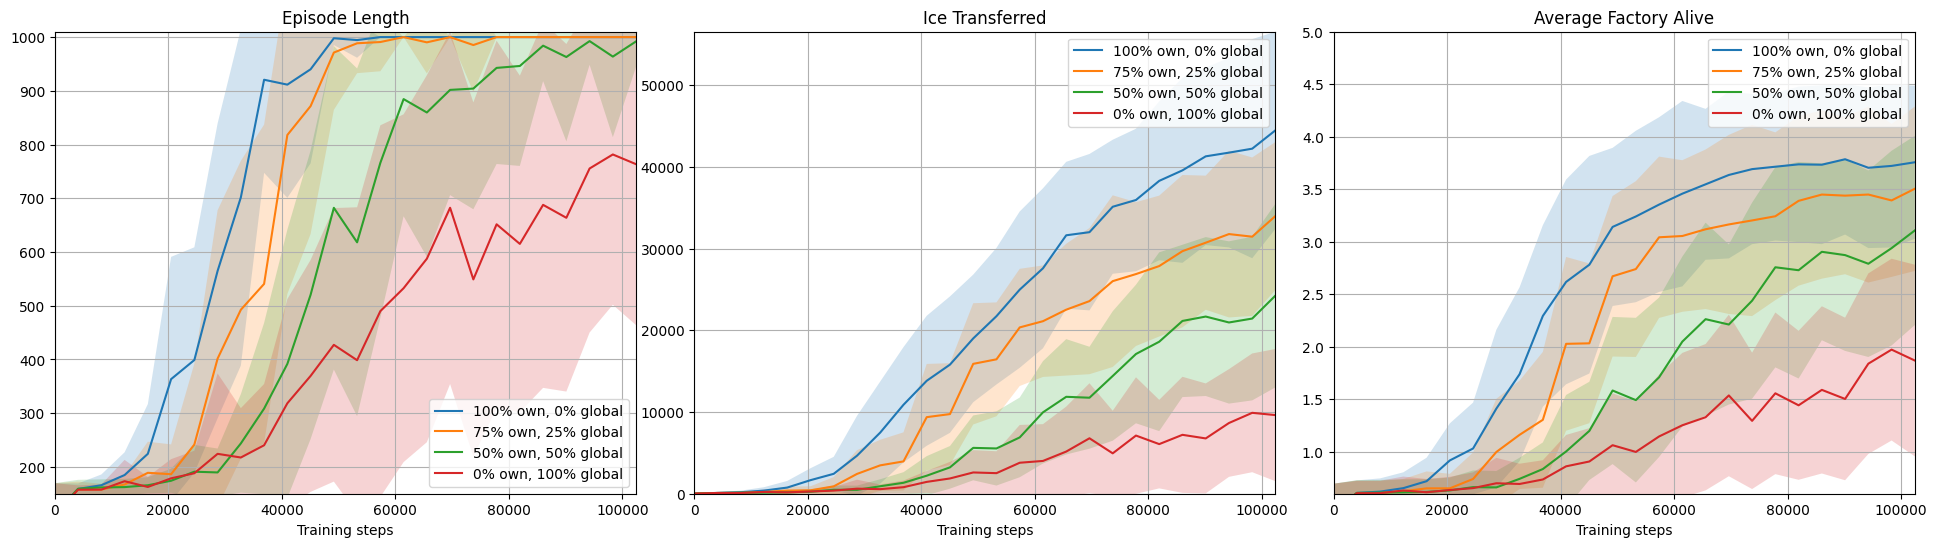
\includegraphics[width=1\linewidth]{images/results_hybrid/reward_assignment/combined.png}
    \captionsetup{justification=justified, singlelinecheck=false, width=1\linewidth, labelfont=bf} 
    \caption[]{Plot comparing the performance of different percentages of global and local rewards in terms of the length of the episodes, ice transferred by units, and number of active factories. In addition to the test variants, the global and completely separate trajectory variants are also present. Mixing in global rewards seems to hinder performance.}
    \label{fig:hybrid_results/reward_assignment/combined}
\end{figure}

\begin{table}[htbp]
    \footnotesize
    \renewcommand{\arraystretch}{1.2}%
    \begin{tabularx}{\textwidth}{|X|C{2.3cm}|C{2.3cm}|C{2.0cm}|C{2.0cm}|}
        \hline
\multicolumn{1}{|Y|}{\textbf{Group Name}} & \textbf{Final Ice Transferred} & \textbf{Final Episode Length} & \textbf{10\% of Episodes Finished by} & \textbf{95\% of Episodes Finished by} \\
        \hline
100\% own, 0\% global & 44,472 (12,065) & 1,000 (0) & 28,672 steps & 49,152 steps \\
75\% own, 25\% global & 33,985 (9,059) & 1,000 (0) & 28,672 steps & 57,344 steps \\
50\% own, 50\% global & 24,244 (11,238) & 992 (47) & 45,056 steps & 94,208 steps \\
0\% own, 100\% global & 9,614 (8,094) & 763 (300) & 53,248 steps & - \\
        \hline
    \end{tabularx}
    \medskip
    \captionsetup{justification=justified, singlelinecheck=false, width=1\linewidth, labelfont=bf} 
    \caption{Table comparing the performance of different global and local rewards percentages. The metrics featured include the amount of ice transferred by units and the length of the episodes in the evaluation phase following the last training cycle. The table also contains the observed environment steps needed until the model reaches the maximum episode length in the specified percentage of evaluation environments. In addition to the test variants, the global and completely separate trajectory variants are also present.}
    \label{tab:hybrid_results/reward_assignment/combined}
\end{table}


\subsection{Comparison with other works}
\label{subsec:comparison}

\noindent As previously stated in this section, the training objectives in the experiments demonstrating trajectory separation were focused on achieving the maximum episode length, which can be accomplished by keeping at least one factory alive from both players. Factories have a lichen watering action (\autoref{sec:wincondition}), which is used to determine the winner if both players successfully maintain their factories until the maximum duration of the episode. In the experiments, we masked out (\autoref{subsec:actions}) this watering action in order to achieve faster convergence. This decision was made since watering can reduce the potential lifespan of a factory. Consequently, in order to conduct a comparative analysis between our approach and state-of-the-art solutions, it was necessary to enable lichen watering. As a result, we proceeded to train a slightly different version of our model. We used trajectory separation (\autoref{sec:trajectory-separation}) without any kind of grouping rule (\autoref{subsec:grouping}) or trajectory sample reduction (\autoref{subsec:tsr}). Given that the other solutions gave rewards for growing lichen, we made adjustments to the reward functions so that the factories received rewards proportional to the number of lichen tiles present on the board at the end of the episode. Lichen can only be grown on rubbleless tiles; thus, we also rewarded units after clearing away rubble next to factories and lichen tiles. We measured how long it took for the modified model to learn how to keep the factories alive up to the maximum episode length. The performance of the modified model compared to the original can be observed in \autoref{fig:hybrid_results/lichen_vs_ts/combined} and \autoref{tab:hybrid_results/lichen_vs_ts/combined}. Even though enabling and rewarding the watering action caused a slight decrease in performance, the model still managed to learn how to transport sufficient ice to factories. It also learned how to successfully grow lichen, as can be seen in \autoref{fig:hybrid_results/lichen/combined}.

\begin{figure}[htbp]
    \centering
    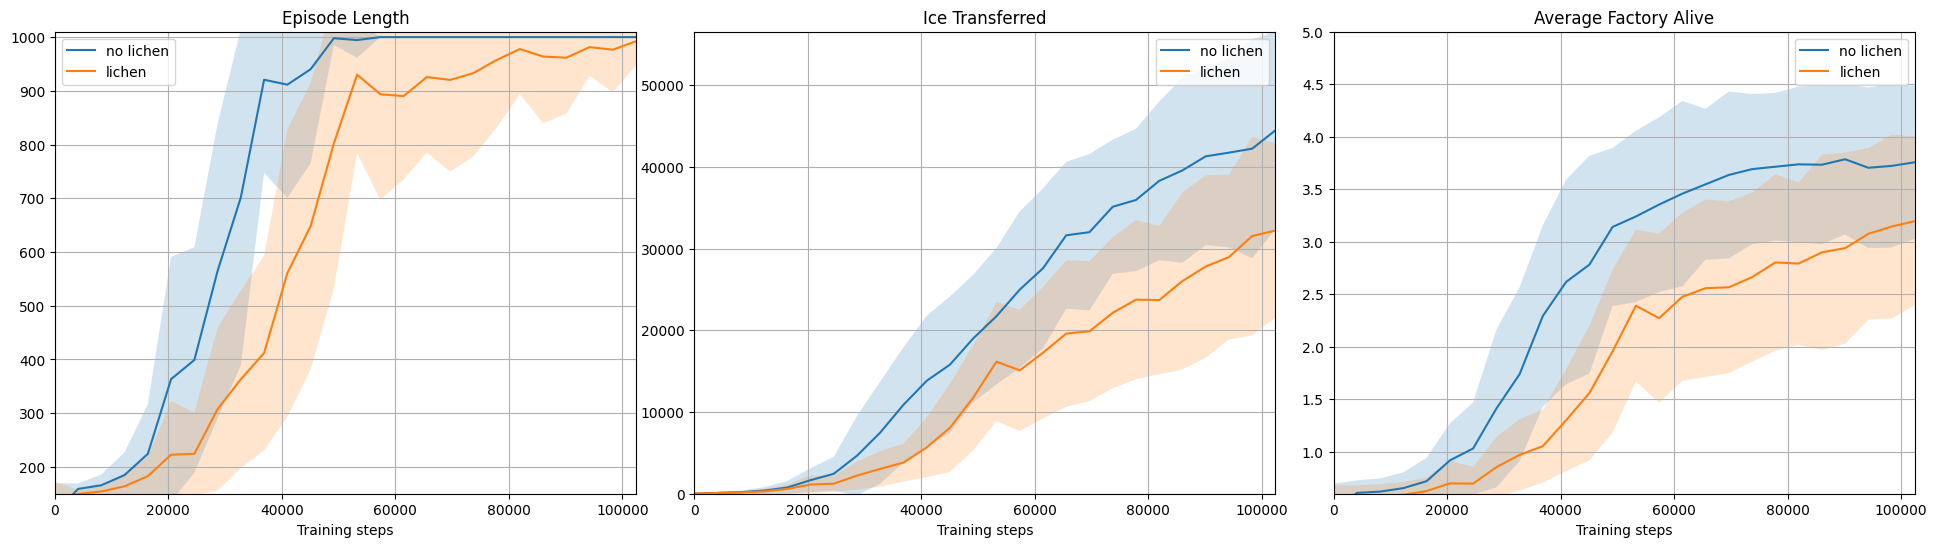
\includegraphics[width=1\linewidth]{images/results_hybrid/lichen_vs_ts/combined.png}
    \captionsetup{justification=justified, singlelinecheck=false, width=1\linewidth, labelfont=bf} 
    \caption[]{Plot comparing the performance of the new lichen-enabled model to the original in terms of the length of the episodes, ice transferred by units, and number of active factories. While lichen watering degrades performance, the goal of reaching the maximum episode length is still achieved at the end of the observed step range.}
    \label{fig:hybrid_results/lichen_vs_ts/combined}
\end{figure}

\begin{table}[htbp]
    \footnotesize
    \renewcommand{\arraystretch}{1.2}%
    \begin{tabularx}{\textwidth}{|X|C{2.3cm}|C{2.3cm}|C{2.0cm}|C{2.0cm}|}
        \hline
\multicolumn{1}{|Y|}{\textbf{Group Name}} & \textbf{Final Ice Transferred} & \textbf{Final Episode Length} & \textbf{10\% of Episodes Finished by} & \textbf{95\% of Episodes Finished by} \\
        \hline
no lichen & 44,472 (12,065) & 1,000 (0) & 28,672 steps & 49,152 steps \\
lichen & 32,199 (10,670) & 992 (45) & 40,960 steps & 102,400 steps \\
        \hline
    \end{tabularx}
    \medskip
    \captionsetup{justification=justified, singlelinecheck=false, width=1\linewidth, labelfont=bf} 
    \caption{Table comparing the performance of the new lichen-enabled model to the original. The metrics featured include the amount of ice transferred by units and the length of the episodes in the evaluation phase following the last training cycle. The table also contains the observed environment steps needed until the model reaches the maximum episode length in the specified percentage of evaluation environments. In addition to the test variants, the global and completely separate trajectory variants are also present. The lichen-enabled variant managed to reach the desired 95\% of completed episodes by the end of the observed step range.}
    \label{tab:hybrid_results/lichen_vs_ts/combined}
\end{table}

\begin{figure}[htbp]
    \centering
    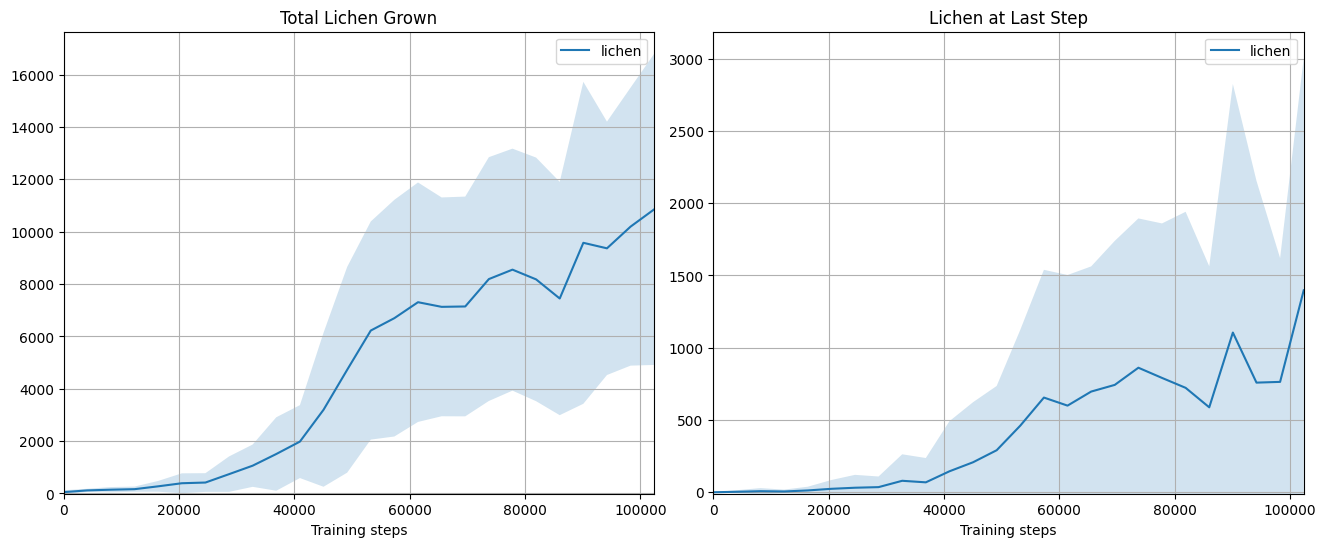
\includegraphics[width=1\linewidth]{images/results_hybrid/lichen/combined.png}
    \captionsetup{justification=justified, singlelinecheck=false, width=1\linewidth, labelfont=bf} 
    \caption[]{Plot showcasing the amount of total lichen grown and the amount of lichen at the end of the episodes. In addition to learning how to reach the maximum episode length (\autoref{fig:hybrid_results/lichen_vs_ts/combined}), the agent demonstrated the ability to solve a secondary task, as shown by the ascending lines.}
    \label{fig:hybrid_results/lichen/combined}
\end{figure}

\bigskip

\noindent We wanted to compare our solution to the top-performing submissions in the Lux AI competition. The basis of our comparison is how long it took for the different models to reach a state where they could keep the factories alive until the maximum episode length in most environments. In our case, this goal was 95\% of episodes. Unfortunately, the leaderboards were predominantly controlled by rule-based methods, resulting in very few RL-based submissions that could be used for a comparative analysis. Many refrained from sharing their work, and in lots of cases where they did share it, their trained models or training metrics were not made publicly available. The only somewhat reliable source we could find was FLG's submission (\cite{ferdinand}), which was somewhat similar to the pixel-to-pixel architecture we started with. Their training objective during the initial "set-up phase" was comparable to ours, which aimed to teach the agent fundamental aspects of the game, such as gathering resources. The duration of their training in terms of time and steps was outlined; however, we are not sure what their stopping criteria were. Consequently, for the purpose of our comparison, we will assume that the stopping criterion used in the referenced submission was identical to our own. In addition, we included a baseline solution provided by the competition organizers (\cite{luxai_s2-baseline-source}). The comparison can be seen in \autoref{tab:other-work-comparisons}. Our approach massively outperformed both the baseline and the FLG's submission in every single one of our metrics. We managed to reach the maximum episode length in 95\% of the environments by step 102,400. In comparison, the baseline model required 1.4 million steps to reach the same milestone, while the submission of FLG was trained for 65 million steps. Given that we utilized a larger value for the hyperparameter "number of epochs" compared to the baseline, resulting in faster training, we believed it was necessary to account for this difference in our comparison. Having said that, our approach is still 5 times more efficient in terms of weight updates needed. Our approach also yielded significantly reduced model sizes, with a mere 200 thousand trainable parameters, as opposed to 451 thousand and 6.08 million, respectively. We also compared the training times, although it should be noted that the resources used for training the other two solutions remain undisclosed, potentially introducing a bias to the presented values.

\bigskip

% time it took for ours to reach 102k steps:
% 2.143 h
% 2.113 h
% 1.999 h
% avg: 2.085 h

\begin{table}[htbp]
    \footnotesize
    \renewcommand{\arraystretch}{1.2}%
    \begin{threeparttable}
        \begin{tabularx}{\linewidth}{|X|C{2.0cm}|C{2.0cm}|C{2.0cm}|C{2.0cm}|}
            \hline
            \textbf{Solution} & \textbf{Parameters}  & \textbf{Training time} & \textbf{Environment Steps} & \textbf{Training Epochs} \\
            \hline
            Trajectory Separated Hybrid Approach & \textbf{200K} & \textbf{2 hours} & \textbf{102K} & \textbf{250} \\
            Baseline Solution (\cite{luxai_s2-baseline-source}) & 451K & 2 days & 1.4M & 1364 \\
            Best RL Submission (\cite{ferdinand}) & 6.08M & 2 days\tnote{*} & 65M\tnote{*} & ?\tnote{**} \\
            \hline
        \end{tabularx}
        \begin{tablenotes}
            \item[*] exact stopping criterion is not known, only the number of steps the model was trained on and the time of training.
            \item[**] "number of epochs" hyperparameter not provided.
        \end{tablenotes}
        \captionsetup{justification=justified, singlelinecheck=false, width=1\linewidth, labelfont=bf} 
        \caption{Table containing the comparison of our work with other implementations. We included the best-performing reinforcement learning submission of the Lux AI competition and a baseline repository provided by the organizers. Our method outperforms both of them in terms of both training time and observed environment steps needed to reach the designated goal. The table also shows a significant difference in model sizes.}
        \label{tab:other-work-comparisons}
    \end{threeparttable}
\end{table}


\subsection{Model Ablation Study}
\label{subsec:ablation}

\noindent Through the utilization of trajectory separation (\autoref{sec:trajectory-separation}), we achieved a significant acceleration in the training process of our model. However, as previously discussed in \autoref{sec:monolithic-approach} and \autoref{sec:hybrid-approach}, many additional components played an important role in achieving the level of performance described, with certain components being absolutely indispensable. In this subsection, we performed an ablation study on the key methods employed to demonstrate the various factors that can impact reinforcement learning and the potential pitfalls that can arise.

\subsubsection{Weight Initialization}

\noindent The proper initialization of weights plays a crucial role, particularly in the application of algorithms such as Proximal Policy Optimization (\autoref{sec:ppo}). We have provided an overview of the weight initialization structure of our model in \autoref{subsec:ortho} and will delve into this issue further in \autoref{ch:disc-init-is-all-you-need}. In this study, we aim to illustrate the impact of incorrect initialization on the convergence of our trajectory-separated hybrid (\autoref{sec:hybrid-approach}) model. The study involved the examination of two components: the weight initialization scaling in the output layers and an additional scaling applied to the weights after initialization, referred to as "extra scaling". We tested removing the extra scaling from the hidden layers (\textttdb{"no extra hidden layer scaling"}) as well as from all layers (\textttdb{"no extra scaling"}). We also conducted experiments to evaluate the effects of removing any kind of scaling from the actor output layers (\textttdb{"no actor scaling"}), the critic value output layers (\textttdb{"no value scaling"}), and all output layers (\textttdb{"no scaling"}). As presented in \autoref{fig:hybrid_results/ablation_study/combined_init} and \autoref{tab:hybrid_results/ablation_study/combined_init}, the removal of any weight initialization component leads to deterioration of performance. Eliminating all weight-downscaling techniques renders the model incapable of any kind of learning. The main problem with large weights is their effect on the initial policies. A network that exhibits a high degree of bias may not assign equal probabilities to all possible actions, resulting in a decrease in the exploration of different actions and a slower rate of learning. This biased network can sometimes lead to policy collapse, as observed with variant \textttdb{"no actor scaling"}. Interestingly, removing the critic value output's scaling causes even larger performance degradation because the early parts of the training must be spent on training the value network to overcome its inherent bias. As a result, the predicted advantage values, which are essential for the Proximal Policy Optimization (PPO) algorithm, will be inaccurate.

\begin{figure}[htbp]
    \centering
    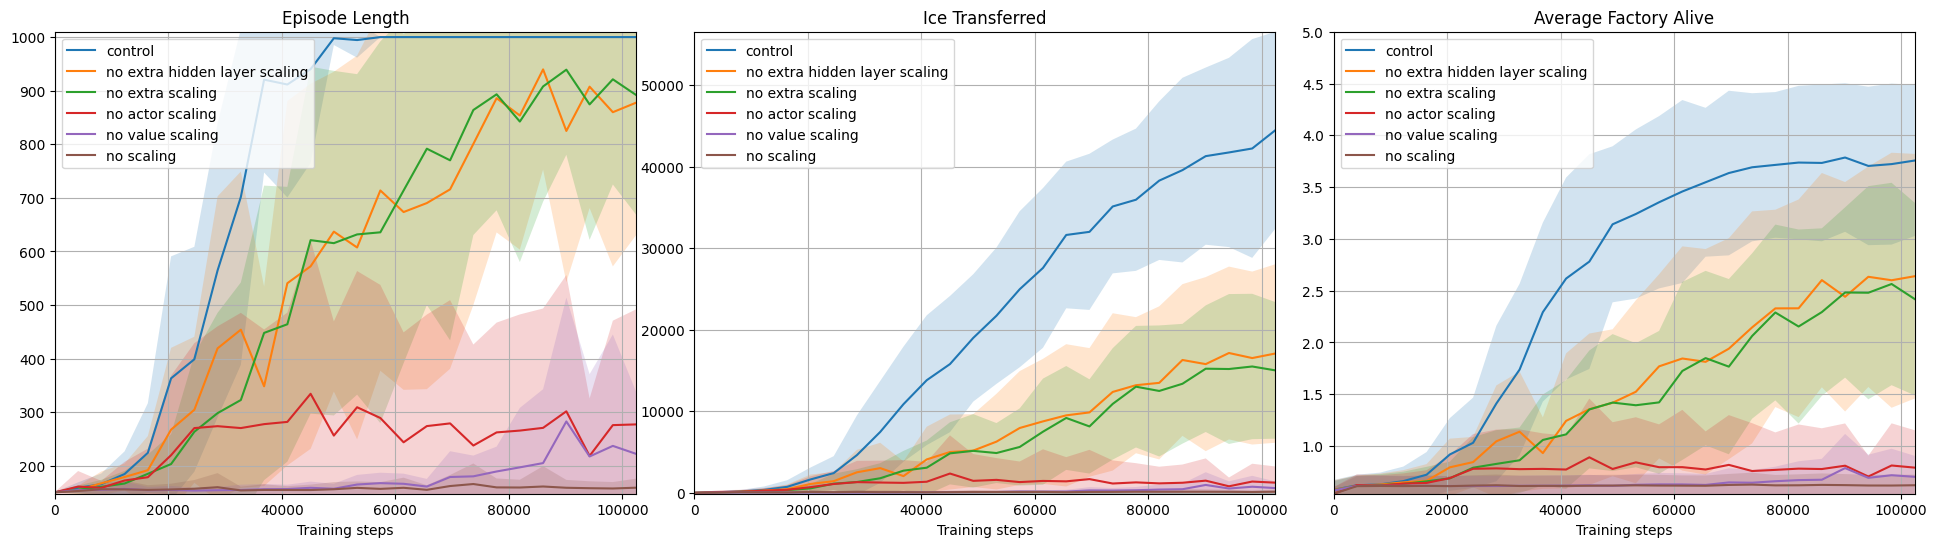
\includegraphics[width=1\linewidth]{images/results_hybrid/ablation_study/combined_init.png}
    \captionsetup{justification=justified, singlelinecheck=false, width=1\linewidth, labelfont=bf} 
    \caption[]{Plot showcasing the difference in performance weight magnitudes can cause in terms of the length of the episodes, ice transferred by units, and number of active factories. Removing any kind of weight downscaling caused a significant performance decrease. Not scaling down the weights of the output layer at all makes training impossible for the model.}
    \label{fig:hybrid_results/ablation_study/combined_init}
\end{figure}

\begin{table}[htbp]
    \footnotesize
    \renewcommand{\arraystretch}{1.2}%
    \begin{tabularx}{\textwidth}{|X|C{2.3cm}|C{2.3cm}|C{2.0cm}|C{2.0cm}|}
        \hline
\multicolumn{1}{|Y|}{\textbf{Group Name}} & \textbf{Final Ice Transferred} & \textbf{Final Episode Length} & \textbf{10\% of Episodes Finished by} & \textbf{95\% of Episodes Finished by} \\
        \hline
control & 44,472 (12,065) & 1,000 (0) & 28,672 steps & 49,152 steps \\
no extra hidden layer scaling & 17,093 (10,944) & 878 (247) & 32,768 steps & - \\
no extra scaling & 15,019 (8,371) & 892 (223) & 36,864 steps & - \\
no actor scaling & 1,255 (1,986) & 277 (215) & 45,056 steps & - \\
no value scaling & 591 (811) & 222 (116) & - & - \\
no scaling & 145 (257) & 159 (17) & - & - \\
        \hline
    \end{tabularx}
    \medskip
    \captionsetup{justification=justified, singlelinecheck=false, width=1\linewidth, labelfont=bf} 
    \caption[]{Table showcasing the difference in performance weight magnitudes can cause. The metrics featured include the amount of ice transferred by units and the length of the episodes in the evaluation phase following the last training cycle. The table also contains the observed environment steps needed until the model reaches the maximum episode length in the specified percentage of evaluation environments. The table clearly shows the decline in performance caused by taking away the weight scalings one by one. None of the studied variants managed to learn how to keep the factories alive until the maximum episode length in most environments.}
    \label{tab:hybrid_results/ablation_study/combined_init}
\end{table}

\subsubsection{Removing Heuristics}

\noindent Our implementation of action masking (\autoref{subsec:mono-actions}) and factory placement (\autoref{subsec:heur-bidding-factory}) introduces a great level of heuristics into the system. Action masking decreases the action space, resulting in faster convergence. Additionally, the strategic placement of factories in close proximity to ice tiles simplifies the environment. Both of these factors play a crucial role, as can be observed in \autoref{fig:hybrid_results/ablation_study/combined_heuristics} and \autoref{tab:hybrid_results/ablation_study/combined_heuristics}. Without the implementation of action masking, the model is presented with an excessive number of potential combinations in its action space, leading to an inability to learn an optimal policy. Consequently, there was no significant increase observed in the \textttdb{"Episode Length"} metric throughout the entire training period. By setting the factory placement to random, the agents can still learn how to transport ice to factories. However, due to the varying distances of ice tiles from factories in each episode, the units are unable to learn how to keep the factories alive within the observed step range.

\begin{figure}[htbp]
    \centering
    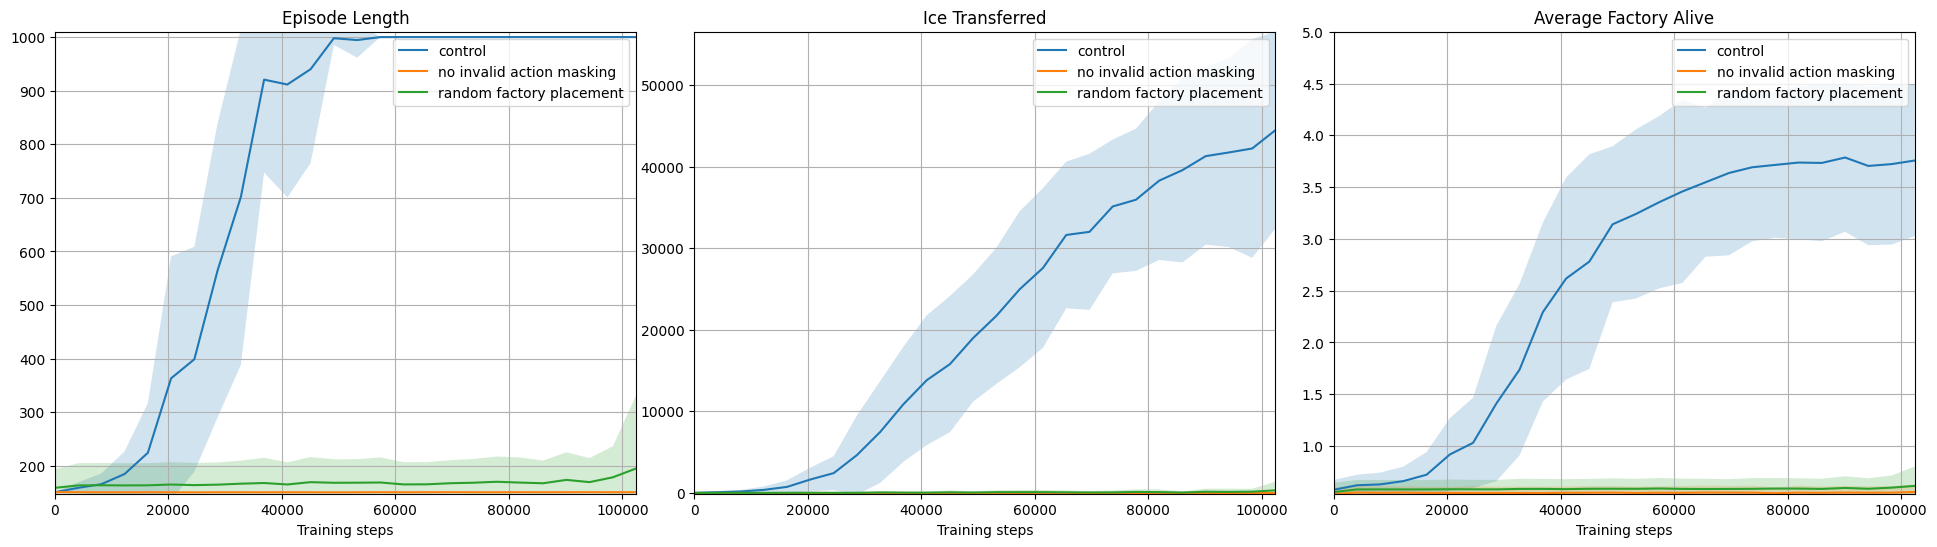
\includegraphics[width=1\linewidth]{images/results_hybrid/ablation_study/combined_heuristics.png}
    \captionsetup{justification=justified, singlelinecheck=false, width=1\linewidth, labelfont=bf} 
    \caption[]{Plot showcasing the difference in performance that removing heuristics causes in terms of the length of the episodes, ice transferred by units, and number of active factories. The elimination of action masking renders training infeasible within the specified step range that we have presented. In addition, the placement of factories at random locations introduces complexity to the environment, resulting in a significant decline in performance.}
    \label{fig:hybrid_results/ablation_study/combined_heuristics}
\end{figure}

\begin{table}[htbp]
    \footnotesize
    \renewcommand{\arraystretch}{1.2}%
    \begin{tabularx}{\textwidth}{|X|C{2.3cm}|C{2.3cm}|C{2.0cm}|C{2.0cm}|}
        \hline
\multicolumn{1}{|Y|}{\textbf{Group Name}} & \textbf{Final Ice Transferred} & \textbf{Final Episode Length} & \textbf{10\% of Episodes Finished by} & \textbf{95\% of Episodes Finished by} \\
        \hline
control & 44,472 (12,065) & 1,000 (0) & 28,672 steps & 49,152 steps \\
no invalid action masking & 0 (0) & 151 (0) & - & - \\
random factory placement & 316 (1,055) & 195 (137) & - & - \\
        \hline
    \end{tabularx}
    \medskip
    \captionsetup{justification=justified, singlelinecheck=false, width=1\linewidth, labelfont=bf} 
    \caption[]{Table showcasing the difference in performance that removing heuristics causes. The metrics featured include the amount of ice transferred by units and the length of the episodes in the evaluation phase following the last training cycle. The table also contains the observed environment steps needed until the model reaches the maximum episode length in the specified percentage of evaluation environments. Without action masking, the units were unable to transfer any ice to factories. Random factory placement still allowed the units to learn that mining and transferring ice are advantageous, but they could not perform said actions optimally.}
    \label{tab:hybrid_results/ablation_study/combined_heuristics}
\end{table}

\subsubsection{Network Regularization}

\noindent In our network, we incorporated two crucial regularization components: batch normalization (\autoref{subsec:batchnorm}) and spectral norm (\autoref{subsec:spectralnorm}). In the following experiment, we tested the necessity of employing both regularization methods. As can be seen in \autoref{fig:hybrid_results/ablation_study/combined_net} and \autoref{tab:hybrid_results/ablation_study/combined_net}, it is apparent that the inclusion of some form of regularization is essential. Removing batch normalization resulted in our model's inability to learn how to reach the maximum episode length within the observed step range. Interestingly, eliminating the spectral norm by itself did not significantly affect performance. Nevertheless, in the absence of batch normalization, the performance deteriorated even further when the spectral norm was removed. This observation suggests that the simultaneous use of both regularization methods may not be necessary. However, including at least one of them is crucial, preferably batch normalization.

\begin{figure}[htbp]
    \centering
    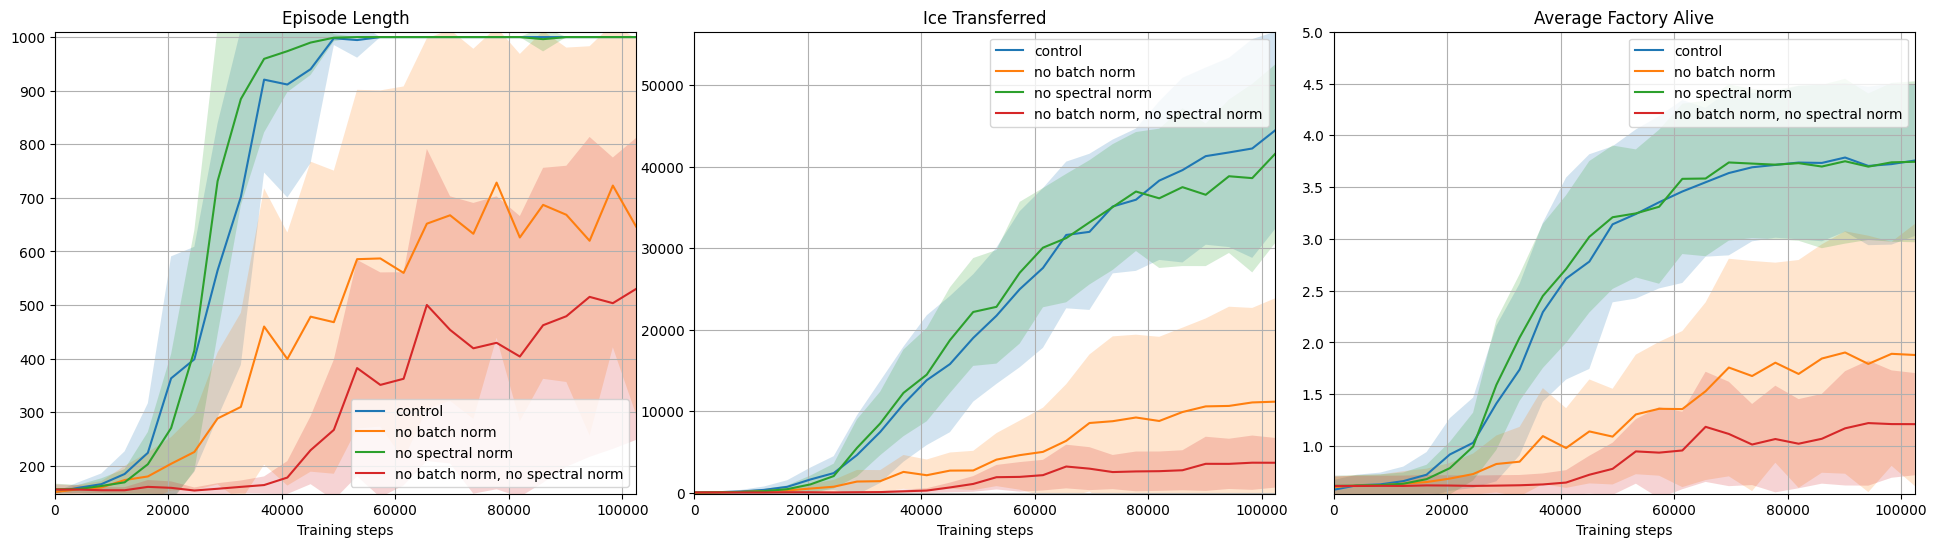
\includegraphics[width=1\linewidth]{images/results_hybrid/ablation_study/combined_net.png}
    \captionsetup{justification=justified, singlelinecheck=false, width=1\linewidth, labelfont=bf} 
    \caption[]{Plot showcasing the difference in performance that removing regularization from our network causes in terms of the length of the episodes, ice transferred by units, and number of active factories. It is clearly visible that batch normalization is the most important regularization component. However, if there is no batch normalization utilized in the network, the presence of spectral norm can help mitigate the need for regularization. Removing batch normalization appears to also cause high variance in the observed metrics.}
    \label{fig:hybrid_results/ablation_study/combined_net}
\end{figure}

\begin{table}[htbp]
    \footnotesize
    \renewcommand{\arraystretch}{1.2}%
    \begin{tabularx}{\textwidth}{|X|C{2.3cm}|C{2.3cm}|C{2.0cm}|C{2.0cm}|}
        \hline
\multicolumn{1}{|Y|}{\textbf{Group Name}} & \textbf{Final Ice Transferred} & \textbf{Final Episode Length} & \textbf{10\% of Episodes Finished by} & \textbf{95\% of Episodes Finished by} \\
        \hline
control & 44,472 (12,065) & 1,000 (0) & 28,672 steps & 49,152 steps \\
no batch norm & 11,184 (12,688) & 646 (351) & 53,248 steps & - \\
no spectral norm & 41,611 (10,938) & 1,000 (0) & 28,672 steps & 45,056 steps \\
no batch norm, no spectral norm & 3,696 (3,039) & 530 (282) & 65,536 steps & - \\
        \hline
    \end{tabularx}
    \medskip
    \captionsetup{justification=justified, singlelinecheck=false, width=1\linewidth, labelfont=bf} 
    \caption[]{Table showcasing the difference in performance that removing regularization from our network causes. The metrics featured include the amount of ice transferred by units and the length of the episodes in the evaluation phase following the last training cycle. The table also contains the observed environment steps needed until the model reaches the maximum episode length in the specified percentage of evaluation environments. Removing batch normalization decreases the model's performance significantly, making it unable to learn how to reach the maximum episode length in all environments. Removing spectral norms further degrades performance.}
    \label{tab:hybrid_results/ablation_study/combined_net}
\end{table}
